\documentclass[11pt,a4paper]{article}

% Image mode: pdf.
% Image paths stay relative. In PDF mode, place same-basename PDF conversions
% of the chapter SVG files in the assets/ directory beside this source.

\usepackage{iftex}
\ifPDFTeX
  \PackageError{handout}{This template requires XeTeX or Tectonic}{Compile with xelatex or tectonic.}
\fi

\usepackage[a4paper,top=18mm,bottom=20mm,left=20mm,right=20mm,headsep=6mm]{geometry}
\usepackage{fontspec}
\usepackage{xeCJK}
\usepackage{amsmath}
\usepackage{unicode-math}

% Font settings are intentionally visible in the generated .tex file.
% These defaults target the macOS machine used for the released PDF.
% Change the family names when compiling on another system.
\setmainfont{Songti TC}
\setsansfont{Heiti TC}
\setmonofont{Menlo}
\setCJKmainfont{Songti TC}
\setCJKsansfont{Heiti TC}
\setCJKmonofont{Heiti TC}
\setmathfont{STIX Two Math}
\XeTeXlinebreaklocale "zh"
\XeTeXlinebreakskip=0pt plus 1pt

\usepackage{xcolor}
\definecolor{HandoutBlue}{HTML}{215A91}
\definecolor{HandoutBlueLight}{HTML}{EEF5FC}
\definecolor{HandoutGreen}{HTML}{39715A}
\definecolor{HandoutGreenLight}{HTML}{EFF8F3}
\definecolor{HandoutGold}{HTML}{8A641C}
\definecolor{HandoutGoldLight}{HTML}{FFF8E8}
\definecolor{HandoutInk}{HTML}{253142}
\definecolor{HandoutMuted}{HTML}{667085}

\usepackage{graphicx}
\makeatletter
% Pandoc 3 emits an accessibility `alt` key for raster/PDF images. Older
% graphicx releases do not know that key, so accept it without changing layout.
\@ifundefined{KV@Gin@alt}{\define@key{Gin}{alt}{}}{}
\newsavebox\pandoc@box
\newcommand*\pandocbounded[1]{%
  \sbox\pandoc@box{#1}%
  \Gscale@div\@tempa{\textheight}{\dimexpr\ht\pandoc@box+\dp\pandoc@box\relax}%
  \Gscale@div\@tempb{\linewidth}{\wd\pandoc@box}%
  \ifdim\@tempb\p@<\@tempa\p@\let\@tempa\@tempb\fi
  \ifdim\@tempa\p@<\p@\scalebox{\@tempa}{\usebox\pandoc@box}%
  \else\usebox{\pandoc@box}%
  \fi
}
\makeatother
\usepackage{float}
\floatplacement{figure}{H}
% Pandoc uses LTcaptype=none for uncaptioned longtables. The caption package
% expects that name to exist as a counter even though it is never displayed.
\newcounter{none}
\usepackage{caption}
\captionsetup[figure]{labelformat=empty,labelsep=none,font=small}

\usepackage{booktabs,longtable,array,calc}
\usepackage{etoolbox}
\makeatletter
\patchcmd\longtable{\par}{\if@noskipsec\mbox{}\fi\par}{}{}
\makeatother

\usepackage[most]{tcolorbox}
\tcbuselibrary{breakable,skins}
\newtcolorbox{HandoutLearningMap}{
  enhanced,breakable,colback=HandoutBlueLight,colframe=HandoutBlue,
  boxrule=0.8pt,arc=1.5mm,left=3mm,right=3mm,top=2mm,bottom=2mm,
  before skip=8pt,after skip=10pt
}
\newtcolorbox{HandoutWorkedExample}{
  enhanced,breakable,colback=HandoutGreenLight,colframe=HandoutGreen,
  boxrule=0.65pt,arc=1.5mm,left=3mm,right=3mm,top=2mm,bottom=2mm,
  before skip=8pt,after skip=10pt
}
\newtcolorbox{HandoutSelfCheck}{
  enhanced,breakable,colback=HandoutGoldLight,colframe=HandoutGold,
  boxrule=0.65pt,arc=1.5mm,left=3mm,right=3mm,top=2mm,bottom=2mm,
  before skip=8pt,after skip=10pt
}

\usepackage{titlesec}
\titleformat{\section}{\sffamily\bfseries\Large\color{HandoutBlue}}{}{0pt}{}
\titleformat{\subsection}{\sffamily\bfseries\large\color{HandoutInk}}{}{0pt}{}
\titleformat{\subsubsection}{\sffamily\bfseries\normalsize\color{HandoutInk}}{}{0pt}{}
\titlespacing*{\section}{0pt}{1.4em}{0.55em}
\titlespacing*{\subsection}{0pt}{1.15em}{0.45em}
\titlespacing*{\subsubsection}{0pt}{0.9em}{0.35em}
\setcounter{secnumdepth}{-\maxdimen}

\usepackage{hyperref}
\usepackage{bookmark}
\IfFileExists{xurl.sty}{\usepackage{xurl}}{}
\urlstyle{same}
\hypersetup{
  colorlinks=true,
  linkcolor=HandoutBlue,
  urlcolor=HandoutBlue,
  citecolor=HandoutBlue,
  pdftitle={必化-2 化學式與化學計量},
  pdfsubject={化學},
  pdfcreator={Pandoc with the HighSchooContent LaTeX template}
}

\setlength{\parindent}{0pt}
\setlength{\parskip}{0.55em plus 0.15em minus 0.1em}
\setlength{\emergencystretch}{3em}
\setlength{\LTpre}{0.5em}
\setlength{\LTpost}{0.5em}
\renewcommand{\arraystretch}{1.18}
\providecommand{\tightlist}{%
  \setlength{\itemsep}{0pt}\setlength{\parskip}{0pt}}
\pagestyle{plain}


\begin{document}

\begin{tcolorbox}[
  enhanced,colback=white,colframe=HandoutBlue,boxrule=1.1pt,arc=2mm,
  borderline west={3pt}{0pt}{HandoutBlue},left=5mm,right=4mm,top=4mm,bottom=4mm
]
{\sffamily\small\bfseries\color{HandoutBlue}學生講義}\par
{\sffamily\bfseries\LARGE\color{HandoutInk}必化-2 化學式與化學計量}\par
\vspace{0.35em}{\large 從組成證據寫出化學式，再用守恆、莫耳與能量帳預測反應結果}\par
\vspace{0.45em}{\small\color{HandoutMuted}%
科目：化學
\quad 課程：普通高中必修化學
\quad 版本：學生版｜核心＋理解
\quad 校訂：2026-08-29
}\par
\vspace{0.25em}{\small\color{HandoutMuted}範圍：現行必修化學第二章主線；含化學式、燃燒分析、反應式、限量試劑、氣體計量與反應能量，氧化還原半反應法及赫斯定律留待選修}\par
\end{tcolorbox}


化學式把元素組成壓縮成可計算的符號，化學反應式再把反應前後的物質連成守恆關係。量到樣品質量、吸收管增重、溶液濃度、氣體體積或溫度變化後，就能依序回答三個問題：物質可能是什麼、最多能生成多少、反應會吸收或釋出多少能量。

這套方法直接用於藥品成分分析、燃料與排放估算、食品與礦石純度、工業配料、氣體產率及製程散熱設計。計算的核心是先確認資料代表哪一種量，再用莫耳與守恆把證據連起來。

\textbf{核心問題：}如何由元素比例判定化學式、如何把實驗事實寫成平衡反應式、如何由反應式預測限量試劑與產量，以及如何由溫度資料回推反應熱。

\section{1. 化學式、百分組成與組成分析}\label{ux5316ux5b78ux5f0fux767eux5206ux7d44ux6210ux8207ux7d44ux6210ux5206ux6790}

\subsection{1.1 四種表示方式回答不同問題}\label{ux56dbux7a2eux8868ux793aux65b9ux5f0fux56deux7b54ux4e0dux540cux554fux984c}

\textbf{實驗式}表示化合物中各元素原子數的最簡整數比。例如葡萄糖的分子式為 \(C_6H_{12}O_6\)，其實驗式為 \(CH_2O\)。離子固體與網狀固體沒有一顆一顆獨立的分子，NaCl、\(SiO_2\) 這類化學式表示組成粒子的最簡比例。

\textbf{分子式}表示一個分子中各元素的實際原子數。若實驗式質量為 \(M_{\mathrm{emp}}\)，實測分子莫耳質量為 \(M\)，則

\[
k=\frac{M}{M_{\mathrm{emp}}},\qquad
\text{分子式}=(\text{實驗式})_k,
\]

其中 \(k\) 應在量測誤差內接近正整數。

\textbf{結構式}表示原子之間的連接方式；線段通常代表共價鍵。平面上的線段是連接關係，不等於所有原子都位於同一平面，也不完整呈現鍵角與立體形狀。

\textbf{示性式或縮寫結構式}保留官能基與部分連接資訊，例如乙醇 \(CH_3CH_2OH\) 的 \(-OH\)、乙酸 \(CH_3COOH\) 的 \(-COOH\)。相同分子式若有不同連接方式，稱為\textbf{結構異構物}，其物理與化學性質可能不同。

\begin{figure}
\centering
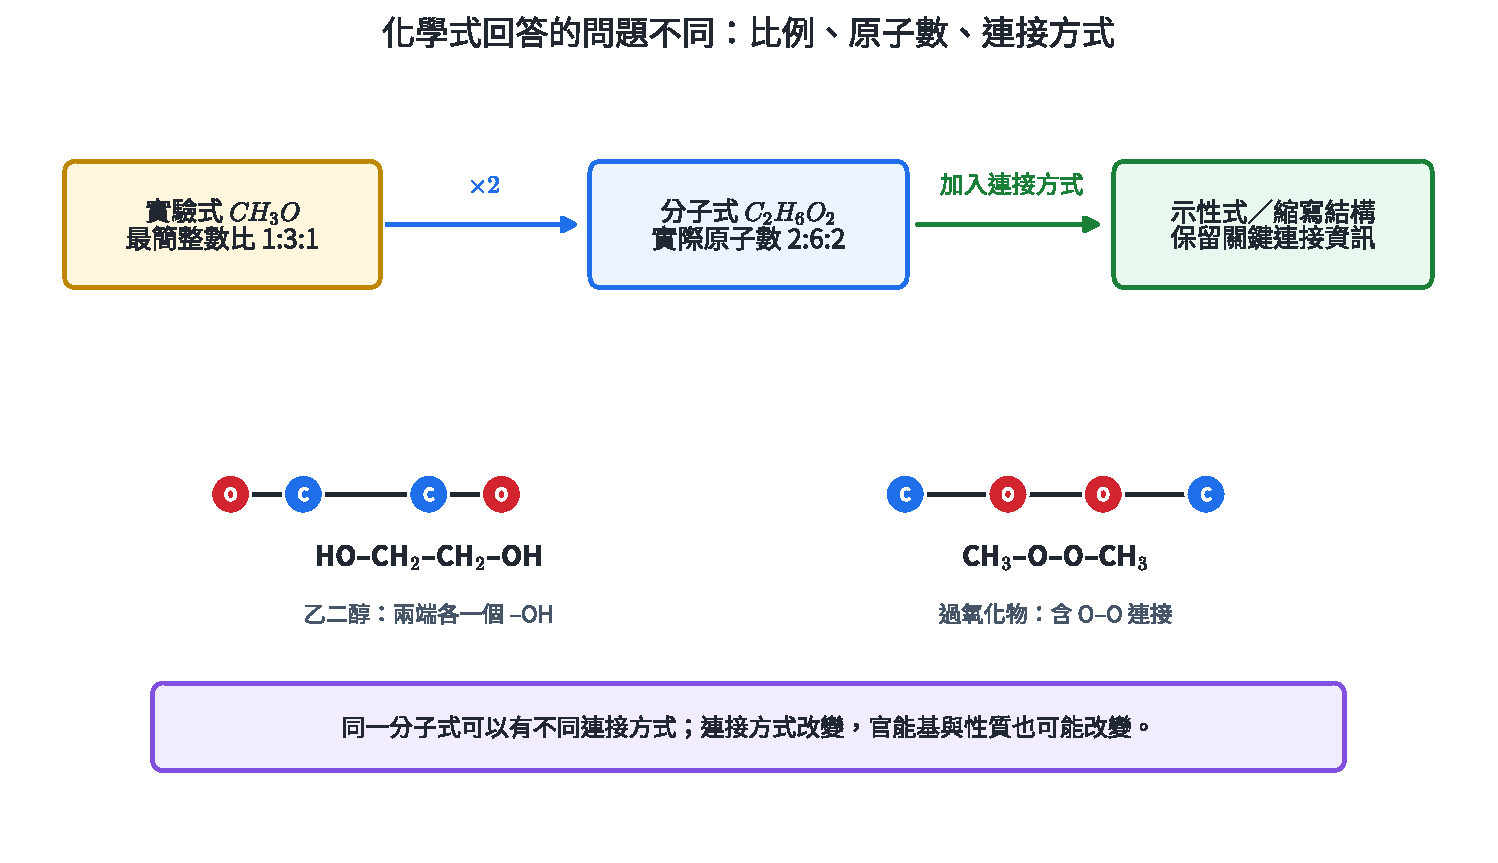
\includegraphics[width=0.96\linewidth,height=\textheight,keepaspectratio,alt={圖 1｜實驗式、分子式與連接方式提供不同層次的資訊；圖中兩種物質皆含 2 C、6 H、2 O。}]{assets/必化-2-化學式資訊層次.pdf}
\caption{圖 1｜實驗式、分子式與連接方式提供不同層次的資訊；圖中兩種物質皆含 2 C、6 H、2 O。}
\end{figure}

化學資料庫、藥品標示與質譜分析常同時使用分子式與結構式：分子式先限制原子數，結構式再指出官能基與可能反應位置。

\subsection{1.2 百分組成把化學式連到可量測的質量}\label{ux767eux5206ux7d44ux6210ux628aux5316ux5b78ux5f0fux9023ux5230ux53efux91cfux6e2cux7684ux8ceaux91cf}

化合物中元素 \(E\) 的質量百分率為

\[
\text{質量百分率}(E)
=\frac{n_E A_E}{M_{\mathrm{formula}}}\times100\%,
\]

其中 \(n_E\) 是一個化學式單位內的 \(E\) 原子數，\(A_E\) 是相對原子質量，\(M_{\mathrm{formula}}\) 是化學式量或莫耳質量。所有元素的百分率總和應在四捨五入誤差內接近 \(100\%\)。

反向由質量資料求實驗式時，依序進行：

\begin{enumerate}
\def\labelenumi{\arabic{enumi}.}
\tightlist
\item
  把各元素質量除以原子量，得到各元素原子的莫耳數。
\item
  所有莫耳數同除以最小值，得到相對比。
\item
  比值若接近 \(1.5,\ 1.33,\ 1.25\) 等簡單分數，整組乘以 \(2,\ 3,\ 4\) 化成最簡整數比。
\item
  把所得實驗式代回原始質量百分率，檢查是否在資料精度內相符。
\end{enumerate}

以百分率為資料時，可假設樣品為 \(100.0\ \mathrm g\)；數值上的百分率便直接成為克數。這只是方便換算的基準，不改變原子比。

\subsection{1.3 燃燒分析：由產物增重追回答案}\label{ux71c3ux71d2ux5206ux6790ux7531ux7522ux7269ux589eux91cdux8ffdux56deux7b54ux6848}

只含 C、H、O 的有機物完全燃燒時，C 全部進入 \(CO_2\)，H 全部進入 \(H_2O\)。若吸收管分別增重 \(m_c\) 與 \(m_w\)，則

\[
n(C)=\frac{m_c}{44.0},\qquad
n(H)=2\frac{m_w}{18.0}.
\]

碳、氫質量為

\[
m(C)=m_c\frac{12.0}{44.0},\qquad
m(H)=m_w\frac{2.0}{18.0}.
\]

樣品已知只含 C、H、O 時，氧可由差值求得：

\[
m(O)=m_{\mathrm{sample}}-m(C)-m(H),\qquad
n(O)=\frac{m(O)}{16.0}.
\]

\begin{figure}
\centering
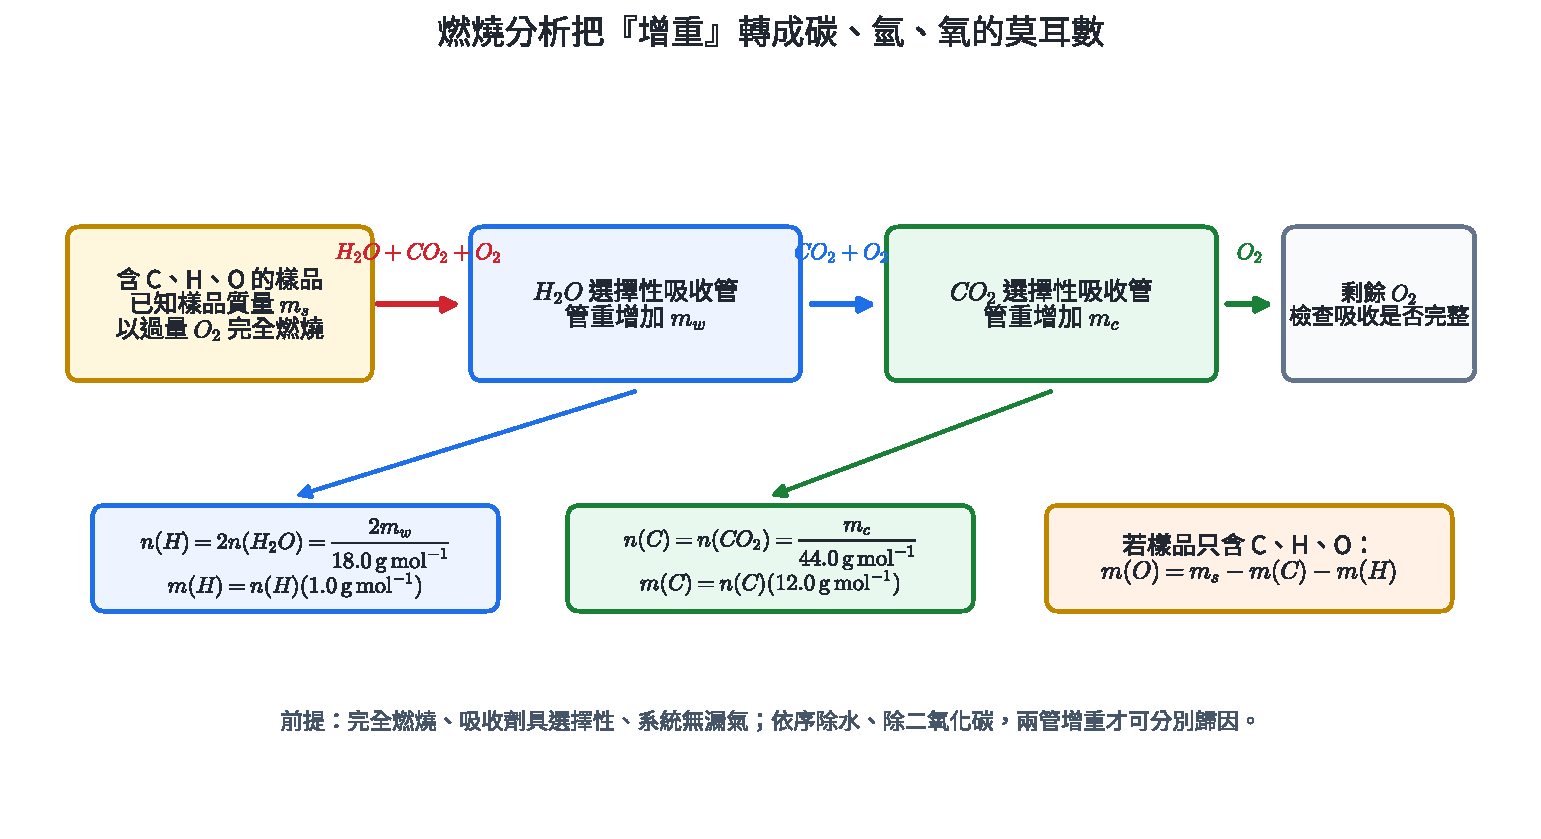
\includegraphics[width=0.98\linewidth,height=\textheight,keepaspectratio,alt={圖 2｜燃燒氣流依序經過除水、除二氧化碳吸收管；各管增重除以相應莫耳質量，再換成 H、C 的莫耳數。}]{assets/必化-2-燃燒分析證據流.pdf}
\caption{圖 2｜燃燒氣流依序經過除水、除二氧化碳吸收管；各管增重除以相應莫耳質量，再換成 H、C 的莫耳數。}
\end{figure}

此推論成立的條件包括：樣品成分範圍已知、燃燒完全、裝置不漏氣、吸收劑具選擇性且吸收完全。若樣品另含 N、S、鹵素或金屬，氧的差值會混入其他元素質量，需要增加獨立分析。

燃燒分析裝置涉及高溫、氧化劑與腐蝕性吸收劑，屬受控儀器分析。實際操作依實驗室風險評估、通風與個人防護規範進行；學生可由已提供的增重資料完成定量推論。

\subsection{1.4 分子式與結構需要額外證據}\label{ux5206ux5b50ux5f0fux8207ux7d50ux69cbux9700ux8981ux984dux5916ux8b49ux64da}

元素比例只能得到實驗式。分子式還需要莫耳質量；結構式更需要化學反應、光譜或其他結構證據。由實驗式 \(CH_2O\) 與莫耳質量 \(180\ \mathrm{g\,mol^{-1}}\) 可確定分子式 \(C_6H_{12}O_6\)，仍不能單靠這兩項資料區分葡萄糖、果糖等結構異構物。

\begin{HandoutWorkedExample}

\subsection{示範 1｜由化學式求百分組成}\label{ux793aux7bc4-1ux7531ux5316ux5b78ux5f0fux6c42ux767eux5206ux7d44ux6210}

求 \(CaCO_3\) 中各元素的質量百分率。取 \(Ca=40.0\)、\(C=12.0\)、\(O=16.0\)。

一莫耳 \(CaCO_3\) 的質量為

\[
M=40.0+12.0+3(16.0)=100.0\ \mathrm{g\,mol^{-1}}.
\]

因此

\[
\%Ca=\frac{40.0}{100.0}\times100\%=40.0\%,
\]

\[
\%C=\frac{12.0}{100.0}\times100\%=12.0\%,\qquad
\%O=\frac{48.0}{100.0}\times100\%=48.0\%.
\]

三者總和為 \(100.0\%\)，與化學式的質量帳一致。

\end{HandoutWorkedExample}

\begin{HandoutWorkedExample}

\subsection{示範 2｜由百分組成求實驗式}\label{ux793aux7bc4-2ux7531ux767eux5206ux7d44ux6210ux6c42ux5be6ux9a57ux5f0f}

某化合物含 C \(52.2\%\)、H \(13.0\%\)、O \(34.8\%\)。求實驗式。

以 \(100.0\ \mathrm g\) 為基準：

\[
n(C)=\frac{52.2}{12.0}=4.35,
\]

\[
n(H)=\frac{13.0}{1.00}=13.0,
\qquad
n(O)=\frac{34.8}{16.0}=2.175.
\]

同除以 \(2.175\) 得

\[
C:H:O=2.00:5.98:1.00\approx2:6:1.
\]

實驗式為 \(C_2H_6O\)。代回可得 C 約 \(52.2\%\)、H 約 \(13.0\%\)、O 約 \(34.8\%\)，符合原始精度。

\end{HandoutWorkedExample}

\begin{HandoutWorkedExample}

\subsection{示範 3｜由化合前後質量求實驗式}\label{ux793aux7bc4-3ux7531ux5316ux5408ux524dux5f8cux8ceaux91cfux6c42ux5be6ux9a57ux5f0f}

\(2.43\ \mathrm g\) 鎂完全反應後得到 \(4.03\ \mathrm g\) 氧化物。求實驗式，取 \(Mg=24.3\)、\(O=16.0\)。

氧的質量為

\[
m(O)=4.03-2.43=1.60\ \mathrm g.
\]

\[
n(Mg)=\frac{2.43}{24.3}=0.100\ \mathrm{mol},\qquad
n(O)=\frac{1.60}{16.0}=0.100\ \mathrm{mol}.
\]

原子莫耳比為 \(1:1\)，實驗式為 \(MgO\)。計算使用的是參與反應的氧質量，因此需以產物質量減去原金屬質量。

\end{HandoutWorkedExample}

\begin{HandoutWorkedExample}

\subsection{示範 4｜燃燒分析與分子式}\label{ux793aux7bc4-4ux71c3ux71d2ux5206ux6790ux8207ux5206ux5b50ux5f0f}

\(0.600\ \mathrm g\) 的 C、H、O 化合物完全燃燒，得到 \(0.880\ \mathrm g\ CO_2\) 與 \(0.360\ \mathrm g\ H_2O\)。其莫耳質量為 \(180\ \mathrm{g\,mol^{-1}}\)，求實驗式與分子式。

\[
n(C)=\frac{0.880}{44.0}=0.0200\ \mathrm{mol},
\]

\[
n(H)=2\frac{0.360}{18.0}=0.0400\ \mathrm{mol}.
\]

碳、氫質量為 \(0.240\ \mathrm g\) 與 \(0.0400\ \mathrm g\)，故

\[
m(O)=0.600-0.240-0.0400=0.320\ \mathrm g,
\]

\[
n(O)=\frac{0.320}{16.0}=0.0200\ \mathrm{mol}.
\]

比值為 \(C:H:O=1:2:1\)，實驗式為 \(CH_2O\)，實驗式質量為 \(30.0\)。再由

\[
k=\frac{180}{30.0}=6
\]

得到分子式 \(C_6H_{12}O_6\)。

\end{HandoutWorkedExample}

\begin{HandoutWorkedExample}

\subsection{示範 5｜分子式相同，結構與性質仍可不同}\label{ux793aux7bc4-5ux5206ux5b50ux5f0fux76f8ux540cux7d50ux69cbux8207ux6027ux8ceaux4ecdux53efux4e0dux540c}

分子式 \(C_2H_6O\) 可寫成 \(CH_3CH_2OH\) 或 \(CH_3OCH_3\)。

\begin{itemize}
\tightlist
\item
  \(CH_3CH_2OH\) 含 \(C-O-H\) 連接，屬醇，可形成較強的分子間氫鍵。
\item
  \(CH_3OCH_3\) 含 \(C-O-C\) 連接，屬醚，沒有 \(O-H\) 鍵。
\end{itemize}

兩者具有相同的元素百分組成與莫耳質量，燃燒分析無法區分；官能基反應或光譜資料才提供連接方式的證據。

\end{HandoutWorkedExample}

\subsection{1.5 本節練習}\label{ux672cux7bc0ux7df4ux7fd2}

\begin{enumerate}
\def\labelenumi{\arabic{enumi}.}
\tightlist
\item
  求 \(Al_2O_3\) 中 Al 與 O 的質量百分率，取 \(Al=27.0\)、\(O=16.0\)。
\item
  某化合物含 C \(40.0\%\)、H \(6.7\%\)、O \(53.3\%\)。求實驗式。
\item
  \(4.60\ \mathrm g\) 鈉與氯完全反應，產物質量為 \(11.70\ \mathrm g\)。求實驗式，取 \(Na=23.0\)、\(Cl=35.5\)。
\item
  \(0.460\ \mathrm g\) 的 C、H、O 化合物完全燃燒，得到 \(0.880\ \mathrm g\ CO_2\) 與 \(0.540\ \mathrm g\ H_2O\)；莫耳質量為 \(46.0\ \mathrm{g\,mol^{-1}}\)。求實驗式與分子式。
\item
  某物質實驗式為 \(NO_2\)，莫耳質量為 \(92.0\ \mathrm{g\,mol^{-1}}\)。求分子式。
\item
  兩瓶純物質的分子式皆為 \(C_2H_6O\)。寫出兩種可能的示性式，並說明還需哪一類證據才能判斷瓶內結構。
\end{enumerate}

\subsubsection{本節練習解答}\label{ux672cux7bc0ux7df4ux7fd2ux89e3ux7b54}

\begin{enumerate}
\def\labelenumi{\arabic{enumi}.}
\tightlist
\item
  \(M(Al_2O_3)=2(27.0)+3(16.0)=102.0\)，故 Al 為 \(54.0/102.0=52.9\%\)，O 為 \(48.0/102.0=47.1\%\)。
\item
  以 \(100\ \mathrm g\) 計，莫耳比為 \(40.0/12.0:6.7/1.0:53.3/16.0\approx1:2:1\)，實驗式 \(CH_2O\)。
\item
  氯質量 \(=11.70-4.60=7.10\ \mathrm g\)；\(n(Na)=0.200\ \mathrm{mol}\)、\(n(Cl)=0.200\ \mathrm{mol}\)，實驗式 NaCl。
\item
  \(n(C)=0.880/44.0=0.0200\)；\(n(H)=2(0.540/18.0)=0.0600\)。碳、氫質量共 \(0.240+0.060=0.300\ \mathrm g\)，故 \(n(O)=(0.460-0.300)/16.0=0.0100\)。比為 \(2:6:1\)，實驗式 \(C_2H_6O\)；其式量即 \(46.0\)，分子式同為 \(C_2H_6O\)。
\item
  \(M(NO_2)=46.0\)，\(k=92.0/46.0=2\)，分子式 \(N_2O_4\)。
\item
  例如 \(CH_3CH_2OH\) 與 \(CH_3OCH_3\)；以官能基反應、紅外光譜或其他結構分析判定連接方式。
\end{enumerate}

\section{2. 化學反應式與守恆}\label{ux5316ux5b78ux53cdux61c9ux5f0fux8207ux5b88ux6046}

\subsection{2.1 反應式是實驗事實的定量摘要}\label{ux53cdux61c9ux5f0fux662fux5be6ux9a57ux4e8bux5be6ux7684ux5b9aux91cfux6458ux8981}

化學反應式以箭號左側表示反應物、右側表示產物。物態寫在化學式後：\((s)\) 固態、\((l)\) 液態、\((g)\) 氣態、\((aq)\) 水溶液；加熱、催化劑、光照、溫度或壓力等條件標在箭號附近。

一條完整反應式同時包含：

\begin{itemize}
\tightlist
\item
  哪些物質消耗、哪些物質生成。
\item
  物質的狀態與必要反應條件。
\item
  由平衡係數表示的莫耳數變化比例。
\item
  若是離子反應，反應前後總電荷相等。
\end{itemize}

產物身分與反應條件來自實驗證據。配平只調整各物質前的\textbf{係數}；化學式的\textbf{下標}描述該物質本身的固定組成。

\subsection{2.2 配平同時滿足原子數與總電荷守恆}\label{ux914dux5e73ux540cux6642ux6effux8db3ux539fux5b50ux6578ux8207ux7e3dux96fbux8377ux5b88ux6046}

設每種物質前的係數為未知數，要求每一元素在左右兩側的原子總數相同；含離子的反應還要求總電荷相同。係數通常化為最簡整數比。熱化學反應式為了表示每莫耳物質的能量，有時可使用分數係數，並同時縮放 \(\Delta H\)。

\begin{figure}
\centering
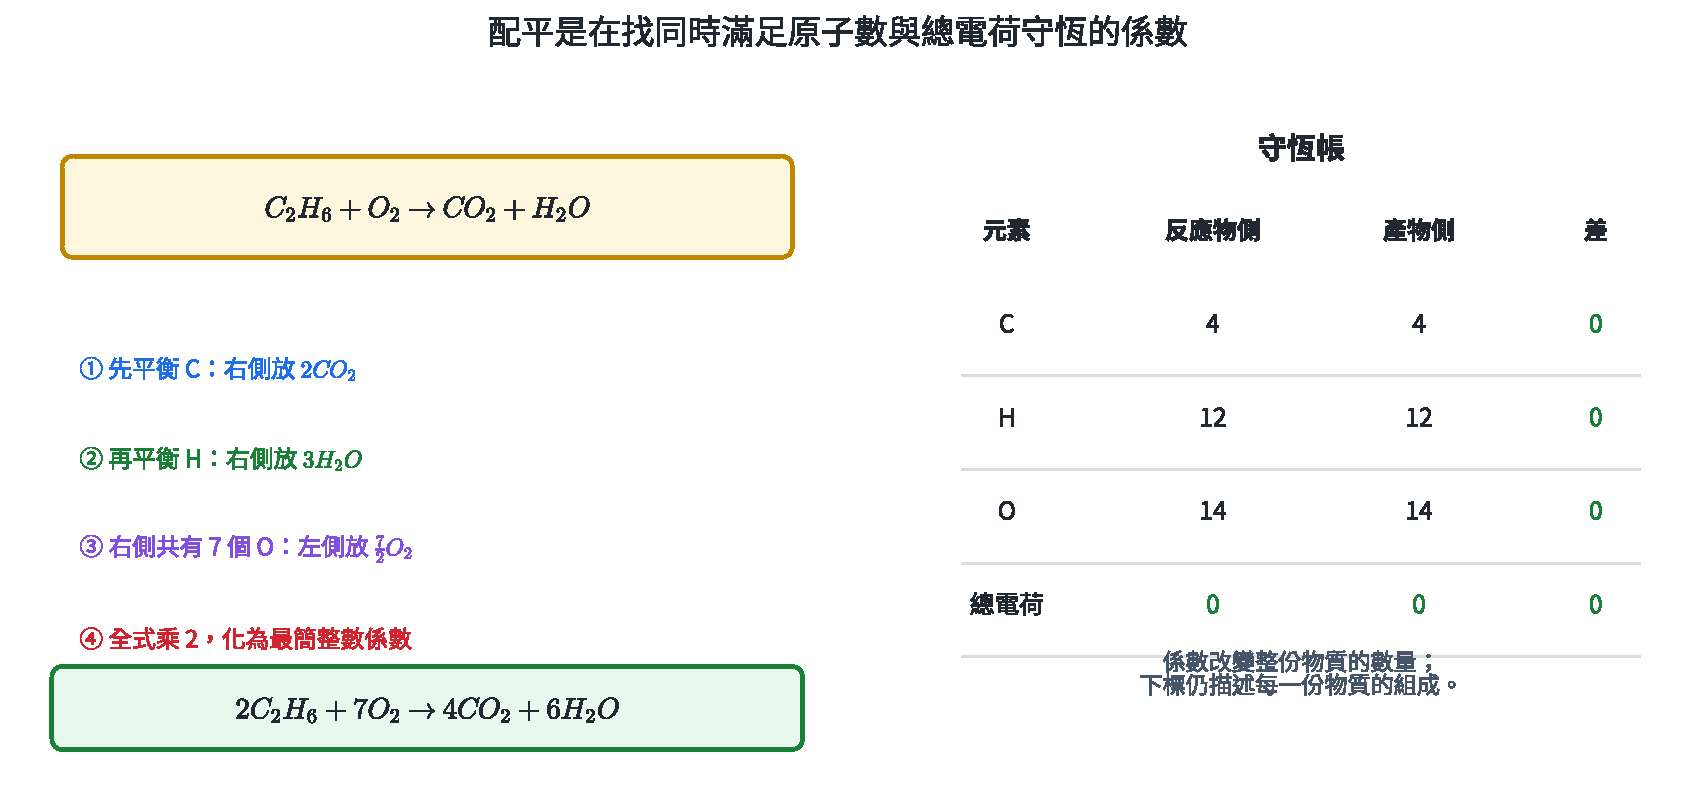
\includegraphics[width=0.96\linewidth,height=\textheight,keepaspectratio,alt={圖 3｜乙烷燃燒的配平過程與守恆帳；左右皆有 4 C、12 H、14 O，總電荷皆為 0。}]{assets/必化-2-反應式配平守恆帳.pdf}
\caption{圖 3｜乙烷燃燒的配平過程與守恆帳；左右皆有 4 C、12 H、14 O，總電荷皆為 0。}
\end{figure}

觀察法適合結構較清楚的反應：先處理只出現在少數物質中的元素，把 H、O 留到後段；多原子離子若反應前後保持整體，可把它視為一組。代數法則為每一物質設係數，逐元素列聯立方程，適合項目多或離子反應。

\subsection{2.3 反應式的資訊邊界}\label{ux53cdux61c9ux5f0fux7684ux8cc7ux8a0aux908aux754c}

平衡係數可直接提供反應進行時的莫耳數、分子數與同溫同壓下氣體體積變化比。結合莫耳質量後，可得到質量關係。

反應速率、實際轉化率、平衡時組成、反應機構與產物純度需要額外資料。\(\Delta H\) 的正負也只描述反應前後能量差，不能單獨決定反應快慢。

\begin{HandoutWorkedExample}

\subsection{示範 6｜觀察法配平金屬氧化物還原}\label{ux793aux7bc4-6ux89c0ux5bdfux6cd5ux914dux5e73ux91d1ux5c6cux6c27ux5316ux7269ux9084ux539f}

配平

\[
Fe_2O_3+CO\rightarrow Fe+CO_2.
\]

\begin{enumerate}
\def\labelenumi{\arabic{enumi}.}
\tightlist
\item
  左側有 2 個 Fe，先在 Fe 前放 2。
\item
  \(Fe_2O_3\) 的 3 個 O 可由 3 個 CO 各再帶入 1 個 O，生成 3 個 \(CO_2\)。
\item
  碳因此也同時平衡。
\end{enumerate}

\[
\boxed{Fe_2O_3+3CO\rightarrow2Fe+3CO_2}
\]

檢查：Fe 為 \(2=2\)，C 為 \(3=3\)，O 為 \(3+3=6=3\times2\)。

\end{HandoutWorkedExample}

\begin{HandoutWorkedExample}

\subsection{示範 7｜代數法配平丙烷燃燒}\label{ux793aux7bc4-7ux4ee3ux6578ux6cd5ux914dux5e73ux4e19ux70f7ux71c3ux71d2}

令

\[
aC_3H_8+bO_2\rightarrow cCO_2+dH_2O.
\]

由 C、H、O 守恆：

\[
3a=c,
\qquad 8a=2d,
\qquad 2b=2c+d.
\]

取最小正整數 \(a=1\)，得 \(c=3\)、\(d=4\)、\(b=5\)：

\[
\boxed{C_3H_8+5O_2\rightarrow3CO_2+4H_2O}.
\]

氧原子檢查：左側 \(10\) 個，右側 \(3(2)+4=10\) 個。

\end{HandoutWorkedExample}

\begin{HandoutWorkedExample}

\subsection{示範 8｜離子反應同時檢查原子與電荷}\label{ux793aux7bc4-8ux96e2ux5b50ux53cdux61c9ux540cux6642ux6aa2ux67e5ux539fux5b50ux8207ux96fbux8377}

鋁在鹼性水溶液中的反應骨架為

\[
Al+OH^-+H_2O\rightarrow Al(OH)_4^-+H_2.
\]

設係數依序為 \(a,b,c,d,e\)。由 Al 與電荷守恆得 \(a=d\)、\(b=d\)；由 O 守恆得 \(b+c=4d\)，故 \(c=3d\)；由 H 守恆得 \(b+2c=4d+2e\)，代入後 \(e=3d/2\)。

取 \(d=2\) 得

\[
\boxed{2Al+2OH^-+6H_2O\rightarrow2Al(OH)_4^-+3H_2}.
\]

左側與右側總電荷皆為 \(-2\)；Al、O、H 原子數也分別相等。

\end{HandoutWorkedExample}

\begin{HandoutWorkedExample}

\subsection{示範 9｜把觀察與條件寫進反應式}\label{ux793aux7bc4-9ux628aux89c0ux5bdfux8207ux689dux4ef6ux5bebux9032ux53cdux61c9ux5f0f}

碳酸氫鈉固體受熱後，得到碳酸鈉固體、二氧化碳與水蒸氣。由物質身分先寫骨架，再配平：

\[
\boxed{2NaHCO_3(s)\xrightarrow{\Delta}Na_2CO_3(s)+CO_2(g)+H_2O(g)}.
\]

檢查 Na \(2=2\)、H \(2=2\)、C \(2=1+1\)、O \(6=3+2+1\)。加熱符號表示反應條件；產氣、冷端凝結水與固體殘留可作為現象證據，產物身分仍以適當檢驗確認。

\end{HandoutWorkedExample}

\subsection{2.4 本節練習}\label{ux672cux7bc0ux7df4ux7fd2-1}

\begin{enumerate}
\def\labelenumi{\arabic{enumi}.}
\tightlist
\item
  配平 \(Al+O_2\rightarrow Al_2O_3\)。
\item
  在 \(MnO_2\) 催化並加熱的條件下，配平 \(KClO_3\rightarrow KCl+O_2\)，並把條件寫在箭號上。
\item
  配平 \(CaBr_2+Na_3PO_4\rightarrow Ca_3(PO_4)_2+NaBr\)。
\item
  配平 \(CrO_4^{2-}+H^+\rightarrow Cr_2O_7^{2-}+H_2O\)，並檢查總電荷。
\item
  對 \(2CO(g)+O_2(g)\rightarrow2CO_2(g)\)，寫出莫耳比、同溫同壓氣體體積比與質量比。
\item
  由原子守恆判定 \(2NH_4NO_3(s)\rightarrow aX(g)+4H_2O(g)+O_2(g)\) 中的 \(a\) 與 \(X\)。
\end{enumerate}

\subsubsection{本節練習解答}\label{ux672cux7bc0ux7df4ux7fd2ux89e3ux7b54-1}

\begin{enumerate}
\def\labelenumi{\arabic{enumi}.}
\tightlist
\item
  \(\boxed{4Al+3O_2\rightarrow2Al_2O_3}\)。
\item
  \(\boxed{2KClO_3(s)\xrightarrow[\Delta]{MnO_2}2KCl(s)+3O_2(g)}\)。
\item
  \(\boxed{3CaBr_2+2Na_3PO_4\rightarrow Ca_3(PO_4)_2+6NaBr}\)。
\item
  \(\boxed{2CrO_4^{2-}+2H^+\rightarrow Cr_2O_7^{2-}+H_2O}\)；左側電荷 \(-4+2=-2\)，右側為 \(-2\)。
\item
  莫耳比與同溫同壓氣體體積比皆為 \(2:1:2\)；質量比為 \(2(28.0):32.0:2(44.0)=56:32:88=7:4:11\)。
\item
  反應物側共有 N 4、H 8、O 6；\(4H_2O+O_2\) 已含 H 8、O 6，故 \(X=N_2\) 且 \(a=2\)。
\end{enumerate}

\clearpage

\section{3. 化學計量、限量試劑與產氣量測}\label{ux5316ux5b78ux8a08ux91cfux9650ux91cfux8a66ux5291ux8207ux7522ux6c23ux91cfux6e2c}

\subsection{3.1 先把已知量轉成莫耳}\label{ux5148ux628aux5df2ux77e5ux91cfux8f49ux6210ux83abux8033}

平衡反應式的係數 \(\nu\) 連接的是莫耳數或粒子數。常用換算為

\[
n=\frac{m}{M},\qquad
n=\frac{N}{N_A},\qquad
n=CV,
\]

其中溶液體積 \(V\) 以 L 代入。氣體可依題目條件使用理想氣體式

\[
n=\frac{PV}{RT},
\]

或使用同溫同壓下已知的莫耳體積。氣體莫耳體積隨溫度與壓力改變，須把條件與數值一起使用。

\begin{figure}
\centering
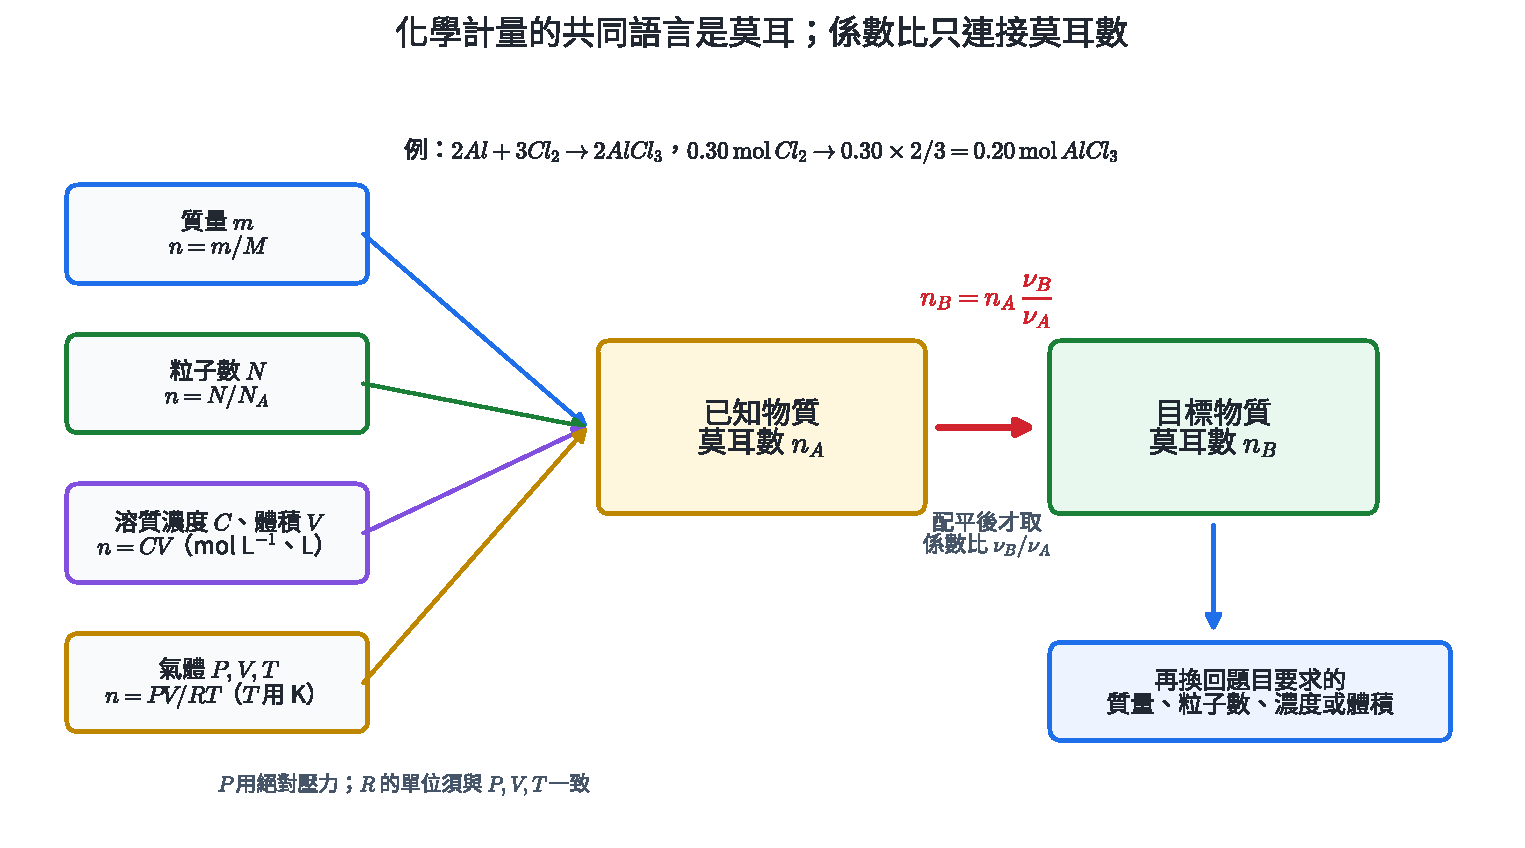
\includegraphics[width=0.98\linewidth,height=\textheight,keepaspectratio,alt={圖 4｜質量、粒子數、溶液與氣體資料先換成莫耳數，再用配平係數比連到目標物；濃度與體積、氣體壓力與溫度須使用相容單位。}]{assets/必化-2-化學計量莫耳橋.pdf}
\caption{圖 4｜質量、粒子數、溶液與氣體資料先換成莫耳數，再用配平係數比連到目標物；濃度與體積、氣體壓力與溫度須使用相容單位。}
\end{figure}

標準計算鏈為

\[
\text{已知量}\rightarrow n_A
\xrightarrow{\nu_B/\nu_A}n_B
\rightarrow\text{目標量}.
\]

每一步保留單位，可以直接看出質量、體積與莫耳是否接在正確的位置。

\subsection{3.2 限量試劑決定最大反應進度}\label{ux9650ux91cfux8a66ux5291ux6c7aux5b9aux6700ux5927ux53cdux61c9ux9032ux5ea6}

對反應

\[
aA+bB\rightarrow cC+dD,
\]

各反應物可支持的反應進度為 \(n(A)/a\)、\(n(B)/b\)。最小值對應\textbf{限量試劑}，最大反應進度為

\[
\xi_{\max}=\min\left(\frac{n(A)}a,\frac{n(B)}b,\ldots\right).
\]

生成量與剩餘量為

\[
n(C)=c\xi_{\max},\qquad
n_{\mathrm{left}}(A)=n_0(A)-a\xi_{\max}.
\]

\begin{figure}
\centering
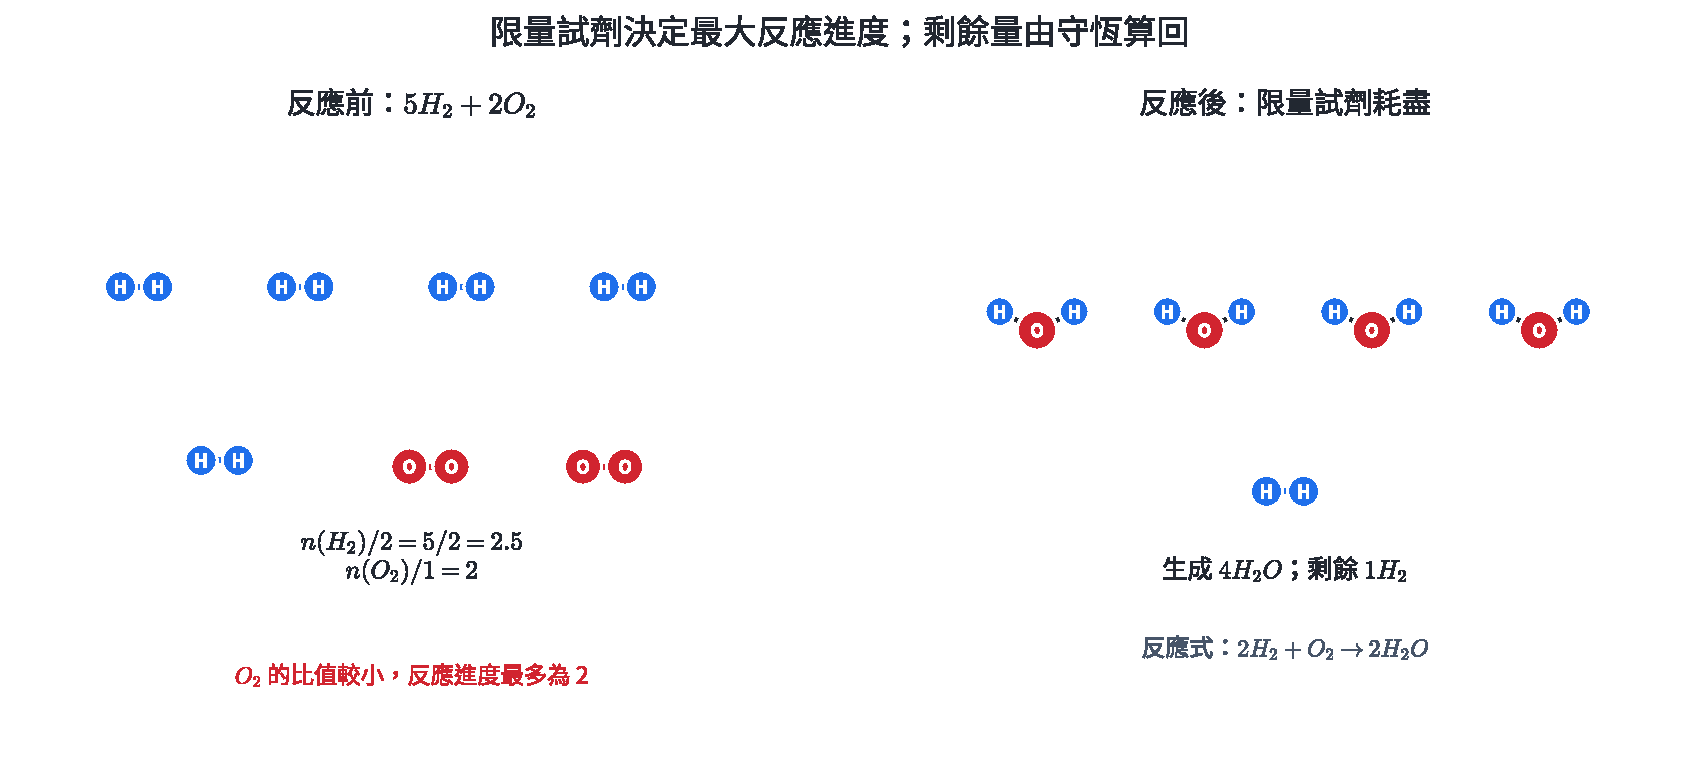
\includegraphics[width=0.94\linewidth,height=\textheight,keepaspectratio,alt={圖 5｜5H\_2 與 2O\_2 反應時，O\_2 先耗盡，生成 4H\_2O 並剩餘 1H\_2；前後 H、O 原子數完全相同。}]{assets/必化-2-限量試劑粒子模型.pdf}
\caption{圖 5｜\(5H_2\) 與 \(2O_2\) 反應時，\(O_2\) 先耗盡，生成 \(4H_2O\) 並剩餘 \(1H_2\)；前後 H、O 原子數完全相同。}
\end{figure}

工業配料、藥物合成與燃燒供氣都使用相同判斷。實際產量常低於理論產量，可用

\[
\text{百分產率}=\frac{\text{實際產量}}{\text{理論產量}}\times100\%
\]

比較製程表現。理論產量由限量試劑決定；實際差異可能來自副反應、未完全反應、轉移損失或量測誤差。

\subsection{3.3 溶液與氣體是常見的計量入口}\label{ux6eb6ux6db2ux8207ux6c23ux9ad4ux662fux5e38ux898bux7684ux8a08ux91cfux5165ux53e3}

溶液先用 \(n=CV\)；若有混合後反應，再依係數判定限量試劑。氣體體積比只有在各氣體溫度與壓力相同時才等於莫耳比。若氣體經水上集氣，乾氣分壓還需由總壓扣除水蒸氣壓；若反應後冷卻造成水凝結，氣相物質種類也會改變。

\subsection{3.4 小量產氣實驗：量測、風險與證據}\label{ux5c0fux91cfux7522ux6c23ux5be6ux9a57ux91cfux6e2cux98a8ux96aaux8207ux8b49ux64da}

鎂與稀鹽酸反應可把固體質量連到氫氣體積：

\[
Mg(s)+2HCl(aq)\rightarrow MgCl_2(aq)+H_2(g).
\]

\begin{figure}
\centering
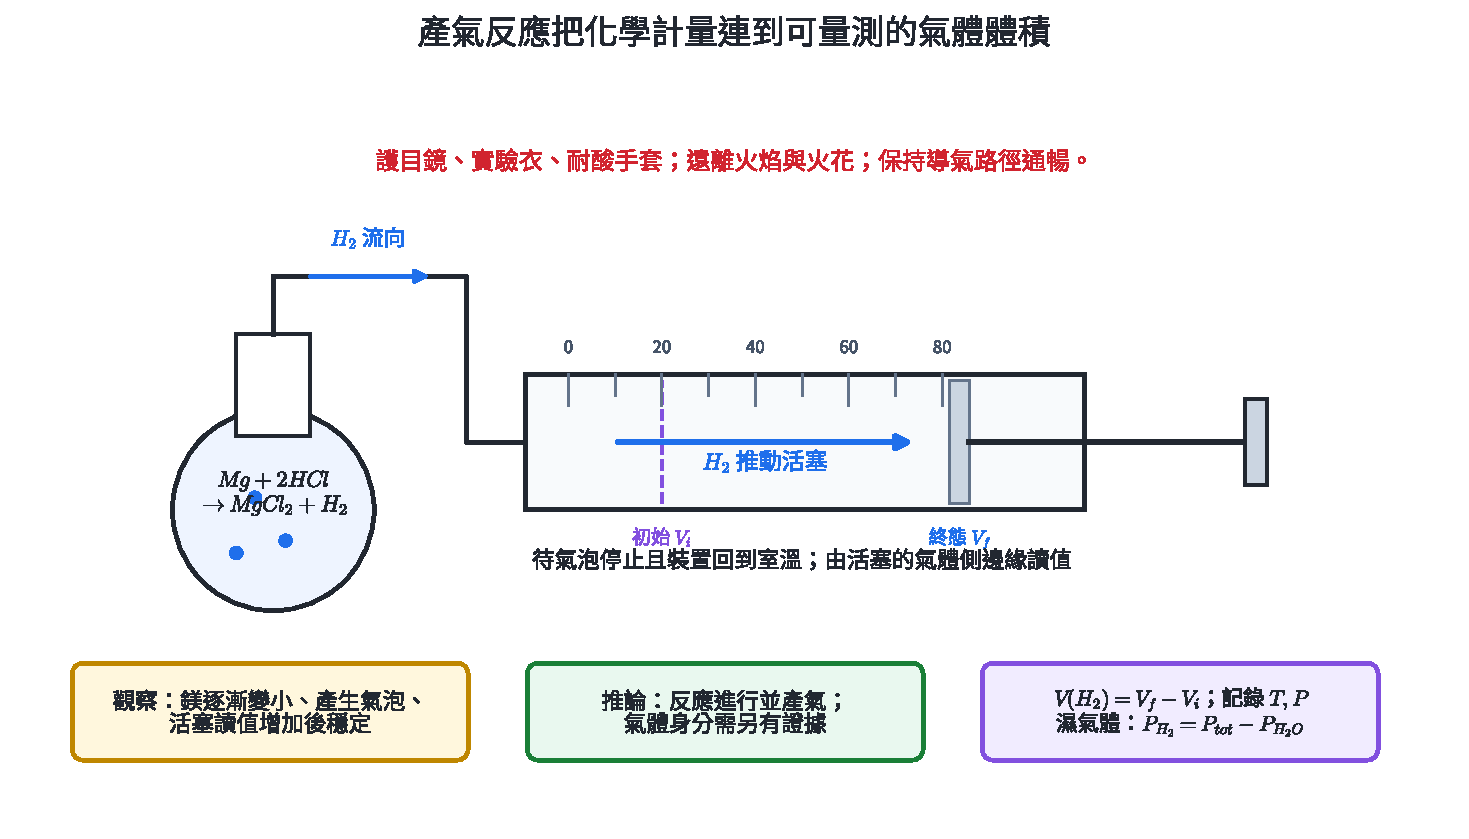
\includegraphics[width=0.96\linewidth,height=\textheight,keepaspectratio,alt={圖 6｜氫氣由反應瓶流入氣體注射筒並推動活塞；回到室溫後由活塞的氣體側邊緣讀值，以 V\_f-V\_i 求產氣體積。}]{assets/必化-2-產氣計量量測.pdf}
\caption{圖 6｜氫氣由反應瓶流入氣體注射筒並推動活塞；回到室溫後由活塞的氣體側邊緣讀值，以 \(V_f-V_i\) 求產氣體積。}
\end{figure}

{\def\LTcaptype{none} % do not increment counter
\begin{longtable}[]{@{}
  >{\raggedright\arraybackslash}p{(\linewidth - 2\tabcolsep) * \real{0.5000}}
  >{\raggedright\arraybackslash}p{(\linewidth - 2\tabcolsep) * \real{0.5000}}@{}}
\toprule\noalign{}
\begin{minipage}[b]{\linewidth}\raggedright
面向
\end{minipage} & \begin{minipage}[b]{\linewidth}\raggedright
實驗處理
\end{minipage} \\
\midrule\noalign{}
\endhead
\bottomrule\noalign{}
\endlastfoot
危害 & 稀鹽酸具腐蝕與刺激性；氫氣易燃；反應產氣使封閉容器升壓 \\
PPE 與環境 & 穿實驗衣、戴護目鏡與耐酸手套；採小量操作；遠離火焰、火花與高溫表面；導氣路徑保持通暢 \\
讀值條件 & 先檢漏並記錄初始讀值 \(V_i\)；氣泡停止、裝置回到室溫後讀取終值 \(V_f\)；同步記錄溫度、壓力與量具解析度 \\
廢液 & 含 \(MgCl_2\) 與可能剩餘酸的水溶液清楚標示，依學校實驗室規範收集或處理 \\
\end{longtable}
}

同一溫度與壓力下，圖示裝置的產氣體積為 \(V_f-V_i\)。固定管路體積在初、末狀態相消；只有儀器校正程序明確指出某段固定體積被包含於單次讀值時，才依該程序另作校正。

觀察與推論分開記錄：

{\def\LTcaptype{none} % do not increment counter
\begin{longtable}[]{@{}
  >{\raggedright\arraybackslash}p{(\linewidth - 4\tabcolsep) * \real{0.3333}}
  >{\raggedright\arraybackslash}p{(\linewidth - 4\tabcolsep) * \real{0.3333}}
  >{\raggedright\arraybackslash}p{(\linewidth - 4\tabcolsep) * \real{0.3333}}@{}}
\toprule\noalign{}
\begin{minipage}[b]{\linewidth}\raggedright
觀察
\end{minipage} & \begin{minipage}[b]{\linewidth}\raggedright
可支持的推論
\end{minipage} & \begin{minipage}[b]{\linewidth}\raggedright
還需控制或補充
\end{minipage} \\
\midrule\noalign{}
\endhead
\bottomrule\noalign{}
\endlastfoot
鎂逐漸變小並持續產生氣泡 & 反應消耗鎂並產生氣體 & 氣體身分需由已知反應與獨立檢驗支持 \\
氣體體積上升後達平臺 & 產氣速率已接近零，某反應物可能耗盡 & 回到同一溫度並確認無漏氣後才能做定量比較 \\
實測體積低於理論值 & 氣體收集不完全或反應／修正條件有差異 & 檢查 \(V_i\)、\(V_f\) 的讀值、漏氣、溫壓、乾濕條件與樣品表面氧化層 \\
\end{longtable}
}

\begin{HandoutWorkedExample}

\subsection{示範 10｜質量到質量的莫耳橋}\label{ux793aux7bc4-10ux8ceaux91cfux5230ux8ceaux91cfux7684ux83abux8033ux6a4b}

\(5.40\ \mathrm g\) Al 與足量 \(Cl_2\) 反應：

\[
2Al+3Cl_2\rightarrow2AlCl_3.
\]

取 \(Al=27.0\)、\(Cl=35.5\)，求 \(AlCl_3\) 質量。

\[
n(Al)=\frac{5.40}{27.0}=0.200\ \mathrm{mol}.
\]

係數比 \(Al:AlCl_3=2:2\)，故 \(n(AlCl_3)=0.200\ \mathrm{mol}\)。\(M(AlCl_3)=133.5\ \mathrm{g\,mol^{-1}}\)，所以

\[
m(AlCl_3)=0.200(133.5)=26.7\ \mathrm g.
\]

\end{HandoutWorkedExample}

\begin{HandoutWorkedExample}

\subsection{示範 11｜溶液濃度到氣體體積}\label{ux793aux7bc4-11ux6eb6ux6db2ux6fc3ux5ea6ux5230ux6c23ux9ad4ux9ad4ux7a4d}

\(100.0\ \mathrm{mL}\)、\(1.50\ \mathrm M\) HCl 與過量 \(CaCO_3\) 反應，在 \(25^\circ\mathrm C\)、\(1.00\ \mathrm{atm}\) 收集乾燥 \(CO_2\)。取此條件氣體莫耳體積為 \(24.5\ \mathrm{L\,mol^{-1}}\)。

\[
CaCO_3+2HCl\rightarrow CaCl_2+H_2O+CO_2.
\]

\[
n(HCl)=(1.50)(0.1000)=0.150\ \mathrm{mol},
\]

\[
n(CO_2)=0.150\times\frac12=0.0750\ \mathrm{mol}.
\]

\[
V(CO_2)=0.0750(24.5)=1.84\ \mathrm L.
\]

體積答案與 \(25^\circ\mathrm C\)、\(1.00\ \mathrm{atm}\) 綁定；改變溫壓便需重新換算。

\end{HandoutWorkedExample}

\begin{HandoutWorkedExample}

\subsection{示範 12｜判斷限量試劑與剩餘量}\label{ux793aux7bc4-12ux5224ux65b7ux9650ux91cfux8a66ux5291ux8207ux5269ux9918ux91cf}

\(2.00\ \mathrm{mol}\ N_2\) 與 \(5.00\ \mathrm{mol}\ H_2\) 依

\[
N_2+3H_2\rightarrow2NH_3
\]

反應。比較

\[
\frac{n(N_2)}1=2.00,
\qquad
\frac{n(H_2)}3=1.667.
\]

\(H_2\) 為限量試劑，\(\xi_{\max}=1.667\ \mathrm{mol}\)。

\[
n(NH_3)=2(1.667)=3.33\ \mathrm{mol},
\]

\[
n_{\mathrm{left}}(N_2)=2.00-1(1.667)=0.333\ \mathrm{mol}.
\]

若取 \(M(NH_3)=17.0\)，理論質量為 \(56.7\ \mathrm g\)。

\end{HandoutWorkedExample}

\begin{HandoutWorkedExample}

\subsection{示範 13｜由產氣資料求礦石純度}\label{ux793aux7bc4-13ux7531ux7522ux6c23ux8cc7ux6599ux6c42ux7926ux77f3ux7d14ux5ea6}

\(2.50\ \mathrm g\) 石灰石樣品與足量酸反應，在 \(25^\circ\mathrm C\)、\(1.00\ \mathrm{atm}\) 得到 \(0.490\ \mathrm L\) 乾燥 \(CO_2\)。假設只有 \(CaCO_3\) 產生 \(CO_2\)，求 \(CaCO_3\) 質量百分率；此條件氣體莫耳體積取 \(24.5\ \mathrm{L\,mol^{-1}}\)。

\[
n(CO_2)=\frac{0.490}{24.5}=0.0200\ \mathrm{mol}.
\]

\(CaCO_3:CO_2=1:1\)，故

\[
m(CaCO_3)=0.0200(100.0)=2.00\ \mathrm g.
\]

\[
\text{純度}=\frac{2.00}{2.50}\times100\%=80.0\%.
\]

結論使用了「其他成分不產生 \(CO_2\)」的模型前提；若雜質也含碳酸鹽，這項計算會高估 \(CaCO_3\)。

\end{HandoutWorkedExample}

\begin{HandoutWorkedExample}

\subsection{示範 14｜限量試劑與固體剩餘量}\label{ux793aux7bc4-14ux9650ux91cfux8a66ux5291ux8207ux56faux9ad4ux5269ux9918ux91cf}

\(6.54\ \mathrm g\) Zn 加入 \(150.0\ \mathrm{mL}\)、\(1.00\ \mathrm M\) HCl：

\[
Zn+2HCl\rightarrow ZnCl_2+H_2.
\]

取 \(M(Zn)=65.4\ \mathrm{g\,mol^{-1}}\)。

\[
n(Zn)=0.100\ \mathrm{mol},\qquad n(HCl)=0.150\ \mathrm{mol}.
\]

\[
\frac{n(Zn)}1=0.100,
\qquad
\frac{n(HCl)}2=0.0750.
\]

HCl 為限量試劑，反應進度為 \(0.0750\ \mathrm{mol}\)。因此生成 \(0.0750\ \mathrm{mol}\ H_2\)，Zn 剩餘

\[
(0.100-0.0750)(65.4)=1.64\ \mathrm g.
\]

\end{HandoutWorkedExample}

\subsection{3.5 本節練習}\label{ux672cux7bc0ux7df4ux7fd2-2}

\begin{enumerate}
\def\labelenumi{\arabic{enumi}.}
\tightlist
\item
  \(4.80\ \mathrm g\) Mg 與足量氧氣依 \(2Mg+O_2\rightarrow2MgO\) 反應。求 \(MgO\) 質量，取 \(Mg=24.0\)、\(O=16.0\)。
\item
  \(50.0\ \mathrm{mL}\)、\(0.200\ \mathrm M\) \(AgNO_3\) 與過量 NaCl 反應生成 AgCl。求 AgCl 質量，取 \(M(AgCl)=143.5\ \mathrm{g\,mol^{-1}}\)。
\item
  同溫同壓下，\(15.0\ \mathrm{mL}\ CH_4\) 依 \(CH_4+2O_2\rightarrow CO_2+2H_2O(g)\) 完全反應。求所需 \(O_2\)、生成 \(CO_2\) 與水蒸氣的體積。
\item
  \(10.0\ \mathrm g\ H_2\) 與 \(64.0\ \mathrm g\ O_2\) 反應生成水。判定限量試劑，求水的理論質量與剩餘反應物質量。
\item
  粒子反應為 \(A_2+3B_2\rightarrow2AB_3\)。起始有 4 個 \(A_2\) 與 9 個 \(B_2\)，求最大可生成的 \(AB_3\) 數與剩餘粒子。
\item
  鎂與足量稀鹽酸反應；反應前氣體注射筒的初始讀值為 \(V_i=2.0\ \mathrm{mL}\)，反應完成並回到相同溫度、壓力後，終值為 \(V_f=52.4\ \mathrm{mL}\)。本題忽略水蒸氣影響，該條件的氣體莫耳體積為 \(24.5\ \mathrm{L\,mol^{-1}}\)。求反應的 Mg 莫耳數與推算質量；若實際秤量為 \(0.0506\ \mathrm g\)，求相對於秤量值的百分差，取 \(M(Mg)=24.3\)。
\end{enumerate}

\subsubsection{本節練習解答}\label{ux672cux7bc0ux7df4ux7fd2ux89e3ux7b54-2}

\begin{enumerate}
\def\labelenumi{\arabic{enumi}.}
\tightlist
\item
  \(n(Mg)=4.80/24.0=0.200\ \mathrm{mol}\)；係數比 \(1:1\)，\(m(MgO)=0.200(40.0)=8.00\ \mathrm g\)。
\item
  \(n(AgNO_3)=0.0500(0.200)=0.0100\ \mathrm{mol}\)；\(Ag^+:AgCl=1:1\)，故 \(m(AgCl)=1.435\ \mathrm g\)。
\item
  同溫同壓下體積比等於係數比 \(1:2:1:2\)，故 \(O_2=30.0\ \mathrm{mL}\)、\(CO_2=15.0\ \mathrm{mL}\)、\(H_2O(g)=30.0\ \mathrm{mL}\)。此結果以水保持氣態為條件。
\item
  \(n(H_2)=5.00\ \mathrm{mol}\)、\(n(O_2)=2.00\ \mathrm{mol}\)；\(n/\nu\) 分別為 \(2.50\)、\(2.00\)，故 \(O_2\) 為限量試劑。生成 \(4.00\ \mathrm{mol}\) 水，即 \(72.0\ \mathrm g\)；剩餘 \(1.00\ \mathrm{mol}\ H_2=2.00\ \mathrm g\)。
\item
  \(4/1=4\)、\(9/3=3\)，故 \(B_2\) 為限量試劑；反應進度為 3，生成 6 個 \(AB_3\)，剩 1 個 \(A_2\)。
\item
  產氣體積為 \(V_f-V_i=52.4-2.0=50.4\ \mathrm{mL}=0.0504\ \mathrm L\)。\(n(H_2)=0.0504/24.5=2.06\times10^{-3}\ \mathrm{mol}\)；由 \(Mg:H_2=1:1\)，\(n(Mg)=2.06\times10^{-3}\ \mathrm{mol}\)，推算 \(m(Mg)=0.0500\ \mathrm g\)。百分差 \(=(0.0500-0.0506)/0.0506\times100\%=-1.2\%\)，表示產氣推算值低約 \(1.2\%\)。
\end{enumerate}

\clearpage

\section{4. 化學反應中的能量變化}\label{ux5316ux5b78ux53cdux61c9ux4e2dux7684ux80fdux91cfux8b8aux5316}

\subsection{4.1 系統、環境與能量流向}\label{ux7cfbux7d71ux74b0ux5883ux8207ux80fdux91cfux6d41ux5411}

研究的反應物與產物稱為\textbf{系統}，其餘可與系統交換能量的部分稱為\textbf{環境}。系統向環境釋出熱量是\textbf{放熱反應}；系統由環境吸收熱量是\textbf{吸熱反應}。

定壓下，反應前後的焓差定義為

\[
\Delta H=H_{\mathrm{products}}-H_{\mathrm{reactants}}.
\]

放熱時 \(H_{\mathrm{products}}<H_{\mathrm{reactants}}\)，故 \(\Delta H<0\)；吸熱時 \(\Delta H>0\)。環境溫度上升通常顯示環境吸熱、系統放熱，兩者的符號需依選定的系統判讀。

\begin{figure}
\centering
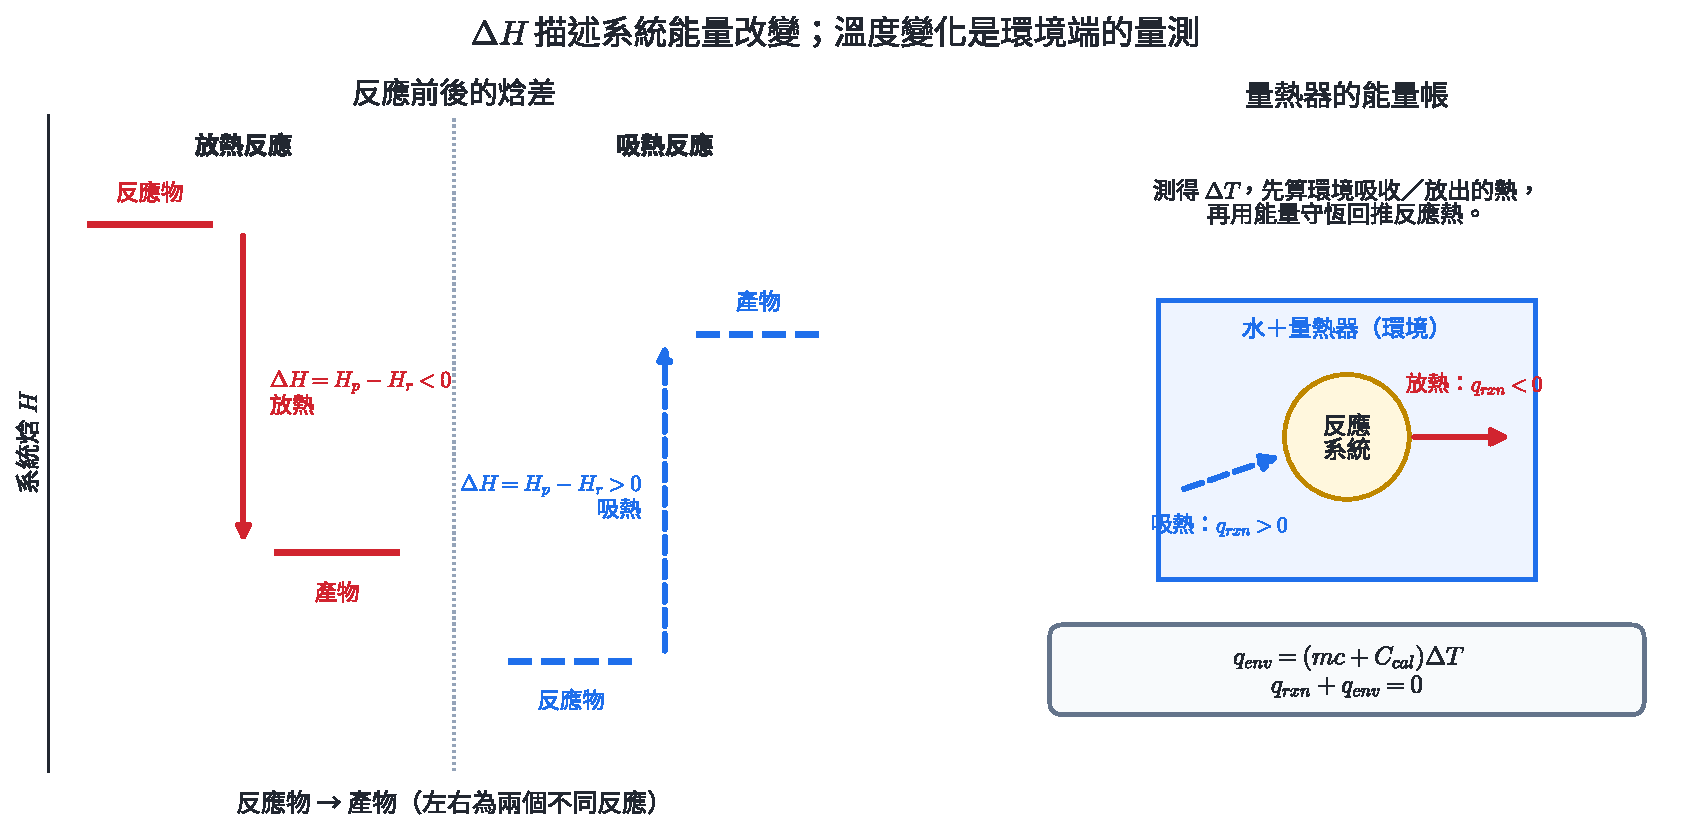
\includegraphics[width=0.98\linewidth,height=\textheight,keepaspectratio,alt={圖 7｜左圖把放熱、吸熱分成兩個反應前後焓階；右圖以箭頭表示熱進出反應系統，量到環境溫度變化後由 q\_\{rxn\}=-q\_\{env\} 回推反應熱。}]{assets/必化-2-反應能量與量熱.pdf}
\caption{圖 7｜左圖把放熱、吸熱分成兩個反應前後焓階；右圖以箭頭表示熱進出反應系統，量到環境溫度變化後由 \(q_{rxn}=-q_{env}\) 回推反應熱。}
\end{figure}

\subsection{4.2 熱化學反應式的係數、方向與物態}\label{ux71b1ux5316ux5b78ux53cdux61c9ux5f0fux7684ux4fc2ux6578ux65b9ux5411ux8207ux7269ux614b}

熱化學反應式須包含配平反應、物態、條件與對應的 \(\Delta H\)。例如

\[
2H_2(g)+O_2(g)\rightarrow2H_2O(l),
\qquad \Delta H=-572\ \mathrm{kJ}.
\]

此數值對應方程式寫出的反應進度：消耗 \(2\ \mathrm{mol}\ H_2\) 並生成 \(2\ \mathrm{mol}\ H_2O(l)\) 時，系統焓降低 \(572\ \mathrm{kJ}\)。

\begin{itemize}
\tightlist
\item
  方程式所有係數乘以 \(r\)，\(\Delta H\) 也乘以 \(r\)。
\item
  反應方向反轉，\(\Delta H\) 大小相同、正負相反。
\item
  物態改變會改變 \(\Delta H\)；生成液態水與水蒸氣的反應熱不同。
\end{itemize}

\(\Delta H\) 不提供反應速率，也不單獨決定常溫下是否能觀察到反應。活化能、碰撞、反應途徑與平衡資料屬另外的模型。

\subsection{4.3 量熱法：先算環境，再回推系統}\label{ux91cfux71b1ux6cd5ux5148ux7b97ux74b0ux5883ux518dux56deux63a8ux7cfbux7d71}

水或溶液吸收的熱可近似為

\[
q_{\mathrm{solution}}=mc\Delta T.
\]

若量熱器本身的熱容量為 \(C_{\mathrm{cal}}\)，則

\[
q_{\mathrm{cal}}=C_{\mathrm{cal}}\Delta T.
\]

在與外界近似絕熱的模型下，

\[
q_{\mathrm{rxn}}+q_{\mathrm{solution}}+q_{\mathrm{cal}}=0.
\]

真實量測需校正量熱器、熱散失、蒸發與溶液比熱差異。報告結果時寫出採用的近似，才能判斷誤差方向。

\begin{HandoutWorkedExample}

\subsection{示範 15｜由能階資料判斷反應熱}\label{ux793aux7bc4-15ux7531ux80fdux968eux8cc7ux6599ux5224ux65b7ux53cdux61c9ux71b1}

某反應的反應物總焓為 \(240\ \mathrm{kJ}\)，產物總焓為 \(100\ \mathrm{kJ}\)。則

\[
\Delta H=100-240=-140\ \mathrm{kJ}.
\]

系統焓降低 \(140\ \mathrm{kJ}\)，為放熱反應；在近似絕熱的量熱器中，環境端會吸收約 \(140\ \mathrm{kJ}\)。

\end{HandoutWorkedExample}

\begin{HandoutWorkedExample}

\subsection{示範 16｜縮放與反轉熱化學反應式}\label{ux793aux7bc4-16ux7e2eux653eux8207ux53cdux8f49ux71b1ux5316ux5b78ux53cdux61c9ux5f0f}

已知

\[
2H_2(g)+O_2(g)\rightarrow2H_2O(l),
\qquad\Delta H=-572\ \mathrm{kJ}.
\]

\(0.500\ \mathrm{mol}\ H_2\) 完全反應時，反應進度是原式的 \(0.500/2=0.250\)，故

\[
\Delta H=(-572)(0.250)=-143\ \mathrm{kJ}.
\]

若把 \(1.00\ \mathrm{mol}\ H_2O(l)\) 分解成元素，先把原式除以 2 再反轉：

\[
H_2O(l)\rightarrow H_2(g)+\frac12O_2(g),
\qquad\Delta H=+286\ \mathrm{kJ}.
\]

\end{HandoutWorkedExample}

\begin{HandoutWorkedExample}

\subsection{示範 17｜物態造成的反應熱差異}\label{ux793aux7bc4-17ux7269ux614bux9020ux6210ux7684ux53cdux61c9ux71b1ux5deeux7570}

同一溫壓下已知

\[
H_2(g)+\frac12O_2(g)\rightarrow H_2O(g),
\qquad\Delta H=-242\ \mathrm{kJ},
\]

\[
H_2(g)+\frac12O_2(g)\rightarrow H_2O(l),
\qquad\Delta H=-286\ \mathrm{kJ}.
\]

兩式反應物相同，液態水的焓比水蒸氣低

\[
286-242=44\ \mathrm{kJ\,mol^{-1}}.
\]

因此水蒸氣凝結成液態水時

\[
H_2O(g)\rightarrow H_2O(l),
\qquad\Delta H=-44\ \mathrm{kJ\,mol^{-1}}.
\]

液態產物多釋出的熱，正是凝結時傳給環境的能量。

\end{HandoutWorkedExample}

\begin{HandoutWorkedExample}

\subsection{示範 18｜由水溫上升求莫耳反應熱}\label{ux793aux7bc4-18ux7531ux6c34ux6eabux4e0aux5347ux6c42ux83abux8033ux53cdux61c9ux71b1}

\(0.100\ \mathrm{mol}\) 燃料在簡化量熱器中完全反應，使 \(500\ \mathrm g\) 水升溫 \(5.00^\circ\mathrm C\)。取 \(c=4.18\ \mathrm{J\,g^{-1}\,K^{-1}}\)，忽略量熱器與散熱。

\[
q_{\mathrm{water}}=(500)(4.18)(5.00)=10450\ \mathrm J=10.45\ \mathrm{kJ}.
\]

水吸熱為正，故反應系統

\[
q_{\mathrm{rxn}}=-10.45\ \mathrm{kJ}.
\]

每莫耳燃料的反應熱為

\[
\Delta H_{\mathrm{mol}}=\frac{-10.45}{0.100}
=-104.5\ \mathrm{kJ\,mol^{-1}}.
\]

\end{HandoutWorkedExample}

\begin{HandoutWorkedExample}

\subsection{示範 19｜把量熱器熱容量納入能量帳}\label{ux793aux7bc4-19ux628aux91cfux71b1ux5668ux71b1ux5bb9ux91cfux7d0dux5165ux80fdux91cfux5e33}

\(0.0200\ \mathrm{mol}\) 反應使 \(50.0\ \mathrm g\) 水與量熱器一同升溫 \(6.00^\circ\mathrm C\)。水比熱 \(4.18\ \mathrm{J\,g^{-1}\,K^{-1}}\)，量熱器熱容量 \(30.0\ \mathrm{J\,K^{-1}}\)。

\[
q_{\mathrm{water}}=(50.0)(4.18)(6.00)=1254\ \mathrm J,
\]

\[
q_{\mathrm{cal}}=(30.0)(6.00)=180\ \mathrm J.
\]

環境共吸收 \(1434\ \mathrm J\)，所以反應釋出相同大小的熱：

\[
\Delta H_{\mathrm{mol}}
=\frac{-1.434\ \mathrm{kJ}}{0.0200\ \mathrm{mol}}
=-71.7\ \mathrm{kJ\,mol^{-1}}.
\]

\end{HandoutWorkedExample}

\subsection{4.4 本節練習}\label{ux672cux7bc0ux7df4ux7fd2-3}

\begin{enumerate}
\def\labelenumi{\arabic{enumi}.}
\tightlist
\item
  冰融化時系統由環境吸熱；甲烷燃燒時系統向環境放熱。分別寫出 \(\Delta H\) 的正負。
\item
  某反應反應物總焓為 \(320\ \mathrm{kJ}\)、產物總焓為 \(460\ \mathrm{kJ}\)。求 \(\Delta H\) 並判斷能量流向。
\item
  已知 \(N_2+3H_2\rightarrow2NH_3\)，\(\Delta H=-92.4\ \mathrm{kJ}\)。生成 \(0.500\ \mathrm{mol}\ NH_3\) 時的 \(\Delta H\) 為何？分解 \(1.00\ \mathrm{mol}\ NH_3\) 時又為何？
\item
  生成 \(1\ \mathrm{mol}\ H_2O(l)\) 比生成 \(1\ \mathrm{mol}\ H_2O(g)\) 多放出 \(44\ \mathrm{kJ}\)。比較兩者焓的高低，並寫出凝結反應的 \(\Delta H\)。
\item
  \(0.0500\ \mathrm{mol}\) 反應使 \(250\ \mathrm g\) 水升溫 \(3.20^\circ\mathrm C\)。取 \(c=4.18\ \mathrm{J\,g^{-1}\,K^{-1}}\) 且忽略其他熱容量，求莫耳反應熱。
\item
  某反應 \(\Delta H=-80\ \mathrm{kJ}\)。列出仍需額外資料才能判定的兩項：反應速率、平衡轉化率、反應前後焓差、對應方程式反應進度。
\end{enumerate}

\subsubsection{本節練習解答}\label{ux672cux7bc0ux7df4ux7fd2ux89e3ux7b54-3}

\begin{enumerate}
\def\labelenumi{\arabic{enumi}.}
\tightlist
\item
  融化吸熱，\(\Delta H>0\)；燃燒放熱，\(\Delta H<0\)。
\item
  \(\Delta H=460-320=+140\ \mathrm{kJ}\)，系統由環境吸收能量。
\item
  生成 \(0.500\ \mathrm{mol}\) 是原式反應進度的 \(0.500/2=0.250\)，故 \(\Delta H=-23.1\ \mathrm{kJ}\)。分解 \(1.00\ \mathrm{mol}\ NH_3\) 是原式除以 2 再反轉，\(\Delta H=+46.2\ \mathrm{kJ}\)。
\item
  \(H(H_2O(g))\) 較高；\(H_2O(g)\rightarrow H_2O(l)\) 的 \(\Delta H=-44\ \mathrm{kJ\,mol^{-1}}\)。
\item
  \(q_{water}=(250)(4.18)(3.20)=3344\ \mathrm J=3.344\ \mathrm{kJ}\)，故每莫耳反應熱 \(=-3.344/0.0500=-66.9\ \mathrm{kJ\,mol^{-1}}\)。
\item
  反應速率與平衡轉化率都需額外資料；\(\Delta H\) 已直接給出反應前後焓差，但仍須搭配方程式才能知道其對應反應進度。
\end{enumerate}

\section{5. 分層題與跨節整合題}\label{ux5206ux5c64ux984cux8207ux8de8ux7bc0ux6574ux5408ux984c}

\subsection{基礎題}\label{ux57faux790eux984c}

\subsection{題目 1｜百分組成}\label{ux984cux76ee-1ux767eux5206ux7d44ux6210}

求 \(Mg(OH)_2\) 中 Mg、O、H 的質量百分率。取 \(Mg=24.0\)、\(O=16.0\)、\(H=1.0\)。

\subsection{題目 2｜由百分組成求實驗式}\label{ux984cux76ee-2ux7531ux767eux5206ux7d44ux6210ux6c42ux5be6ux9a57ux5f0f}

某化合物只含 C 與 O，質量百分率分別為 C \(27.3\%\)、O \(72.7\%\)。求實驗式。

\subsection{題目 3｜由實驗式求分子式}\label{ux984cux76ee-3ux7531ux5be6ux9a57ux5f0fux6c42ux5206ux5b50ux5f0f}

某化合物實驗式為 \(C_2H_5O\)，莫耳質量為 \(90.0\ \mathrm{g\,mol^{-1}}\)。求分子式。

\subsection{題目 4｜反應式配平}\label{ux984cux76ee-4ux53cdux61c9ux5f0fux914dux5e73}

配平黃鐵礦焙燒的反應：

\[
FeS_2+O_2\rightarrow Fe_2O_3+SO_2.
\]

\subsection{題目 5｜離子反應守恆}\label{ux984cux76ee-5ux96e2ux5b50ux53cdux61c9ux5b88ux6046}

配平

\[
Al+H^+\rightarrow Al^{3+}+H_2,
\]

並檢查總電荷。

\subsection{應用題}\label{ux61c9ux7528ux984c}

\subsection{題目 6｜燃燒的質量計量}\label{ux984cux76ee-6ux71c3ux71d2ux7684ux8ceaux91cfux8a08ux91cf}

\(12.0\ \mathrm g\) 純碳完全燃燒生成 \(CO_2\)。求所需 \(O_2\) 與生成 \(CO_2\) 的質量。

\subsection{題目 7｜溶液到氣體}\label{ux984cux76ee-7ux6eb6ux6db2ux5230ux6c23ux9ad4}

\(25.0\ \mathrm{mL}\)、\(0.800\ \mathrm M\) HCl 與過量 \(Na_2CO_3\) 反應：

\[
Na_2CO_3+2HCl\rightarrow2NaCl+H_2O+CO_2.
\]

求 \(CO_2\) 莫耳數；在 \(25^\circ\mathrm C\)、\(1.00\ \mathrm{atm}\)，取莫耳體積 \(24.5\ \mathrm{L\,mol^{-1}}\)，再求乾燥 \(CO_2\) 體積。

\subsection{題目 8｜限量試劑}\label{ux984cux76ee-8ux9650ux91cfux8a66ux5291}

\(3.00\ \mathrm{mol}\ CO\) 與 \(1.00\ \mathrm{mol}\ O_2\) 依

\[
2CO+O_2\rightarrow2CO_2
\]

反應。求限量試劑、\(CO_2\) 生成量與過量反應物剩餘量。

\subsection{題目 9｜同溫同壓氣體體積}\label{ux984cux76ee-9ux540cux6eabux540cux58d3ux6c23ux9ad4ux9ad4ux7a4d}

同溫同壓下，\(20.0\ \mathrm{mL}\ N_2\) 與 \(45.0\ \mathrm{mL}\ H_2\) 依

\[
N_2+3H_2\rightarrow2NH_3
\]

完全反應。求生成 \(NH_3\) 與剩餘 \(N_2\) 的體積，假設所有氣體保持相同溫壓。

\subsection{題目 10｜熱化學式縮放}\label{ux984cux76ee-10ux71b1ux5316ux5b78ux5f0fux7e2eux653e}

已知

\[
2SO_2(g)+O_2(g)\rightarrow2SO_3(g),
\qquad\Delta H=-198\ \mathrm{kJ}.
\]

生成 \(0.750\ \mathrm{mol}\ SO_3\) 時的 \(\Delta H\) 為何？將這些 \(SO_3\) 分解回 \(SO_2\) 與 \(O_2\) 時又為何？

\subsection{題目 11｜量熱資料}\label{ux984cux76ee-11ux91cfux71b1ux8cc7ux6599}

\(0.0250\ \mathrm{mol}\) 反應使 \(100.0\ \mathrm g\) 水升溫 \(5.00^\circ\mathrm C\)。取 \(c=4.18\ \mathrm{J\,g^{-1}\,K^{-1}}\) 且忽略散熱與量熱器熱容量，求莫耳反應熱。

\subsection{題目 12｜焓差與環境}\label{ux984cux76ee-12ux7113ux5deeux8207ux74b0ux5883}

某反應反應物總焓為 \(75\ \mathrm{kJ}\)，產物總焓為 \(130\ \mathrm{kJ}\)。求 \(\Delta H\)、判斷吸放熱，並預測近似絕熱時環境的溫度變化方向。

\subsection{跨節整合題}\label{ux8de8ux7bc0ux6574ux5408ux984c}

\subsection{題目 13｜燃料的組成、排放與反應熱}\label{ux984cux76ee-13ux71c3ux6599ux7684ux7d44ux6210ux6392ux653eux8207ux53cdux61c9ux71b1}

某只含 C、H 的燃料 \(0.580\ \mathrm g\) 完全燃燒，得到 \(1.760\ \mathrm g\ CO_2\) 與 \(0.900\ \mathrm g\ H_2O\)。其莫耳質量為 \(58.0\ \mathrm{g\,mol^{-1}}\)。

\begin{enumerate}
\def\labelenumi{\arabic{enumi}.}
\tightlist
\item
  求實驗式與分子式。
\item
  寫出最簡整數係數的完全燃燒反應式。
\item
  \(1.16\ \mathrm g\) 此燃料完全燃燒時，求 \(CO_2\) 質量。
\item
  若第 2 小題反應式所對應的 \(\Delta H=-5752\ \mathrm{kJ}\)，求燃燒 \(1.16\ \mathrm g\) 時的 \(\Delta H\)。
\end{enumerate}

\subsection{題目 14｜水合鹽的組成與脫水能量}\label{ux984cux76ee-14ux6c34ux5408ux9e7dux7684ux7d44ux6210ux8207ux812bux6c34ux80fdux91cf}

\(2.46\ \mathrm g\) 的 \(MgSO_4\cdot xH_2O\) 完全加熱脫水後，留下 \(1.20\ \mathrm g\ MgSO_4\)。取 \(M(MgSO_4)=120\ \mathrm{g\,mol^{-1}}\)、\(M(H_2O)=18.0\ \mathrm{g\,mol^{-1}}\)。

\begin{enumerate}
\def\labelenumi{\arabic{enumi}.}
\tightlist
\item
  求 \(x\)。
\item
  寫出脫水反應式，水在高溫出口以水蒸氣表示。
\item
  若這份樣品脫水的系統焓變為 \(+5.60\ \mathrm{kJ}\)，求每莫耳水合鹽的 \(\Delta H\)。
\end{enumerate}

\subsection{題目 15｜產氫量測、限量試劑與產率}\label{ux984cux76ee-15ux7522ux6c2bux91cfux6e2cux9650ux91cfux8a66ux5291ux8207ux7522ux7387}

\(0.0486\ \mathrm g\) Mg 加入 \(50.0\ \mathrm{mL}\)、\(0.100\ \mathrm M\) HCl。取 \(M(Mg)=24.3\ \mathrm{g\,mol^{-1}}\)，\(25^\circ\mathrm C\)、\(1.00\ \mathrm{atm}\) 的氣體莫耳體積為 \(24.5\ \mathrm{L\,mol^{-1}}\)。

\begin{enumerate}
\def\labelenumi{\arabic{enumi}.}
\tightlist
\item
  判定限量試劑。
\item
  求 \(H_2\) 理論體積。
\item
  校正後實測 \(H_2\) 體積為 \(46.8\ \mathrm{mL}\)，求體積產率。
\item
  寫出一項安全控制，以及「氣體體積上升後達平臺」可支持的一項推論。
\end{enumerate}

\subsection{題目 16｜含雜質石灰石的配料與散熱}\label{ux984cux76ee-16ux542bux96dcux8ceaux77f3ux7070ux77f3ux7684ux914dux6599ux8207ux6563ux71b1}

\(5.00\ \mathrm g\) 石灰石含 \(80.0\%\ CaCO_3\)，其餘為不反應固體。加入 \(60.0\ \mathrm{mL}\)、\(1.00\ \mathrm M\) HCl：

\[
CaCO_3+2HCl\rightarrow CaCl_2+H_2O+CO_2.
\]

\begin{enumerate}
\def\labelenumi{\arabic{enumi}.}
\tightlist
\item
  判定限量試劑。
\item
  求 \(CO_2\) 莫耳數與質量。
\item
  求反應後未反應固體總質量。
\item
  若每反應 \(1.00\ \mathrm{mol}\ CaCO_3\) 的 \(\Delta H=-20.0\ \mathrm{kJ}\)，求此批次的 \(\Delta H\)。
\end{enumerate}

\section{6. 分層題與跨節整合題詳解}\label{ux5206ux5c64ux984cux8207ux8de8ux7bc0ux6574ux5408ux984cux8a73ux89e3}

\subsection{第 1 題}\label{ux7b2c-1-ux984c}

\[
M(Mg(OH)_2)=24.0+2(16.0+1.0)=58.0.
\]

\[
\%Mg=\frac{24.0}{58.0}\times100\%=41.4\%,
\]

\[
\%O=\frac{32.0}{58.0}\times100\%=55.2\%,
\qquad
\%H=\frac{2.0}{58.0}\times100\%=3.45\%.
\]

總和約 \(100.0\%\)。

\subsection{第 2 題}\label{ux7b2c-2-ux984c}

以 \(100.0\ \mathrm g\) 計：

\[
n(C)=\frac{27.3}{12.0}=2.275,
\qquad
n(O)=\frac{72.7}{16.0}=4.544.
\]

同除以 \(2.275\) 得 \(C:O=1.000:1.997\approx1:2\)，實驗式為 \(CO_2\)。代回可得 C 百分率 \(12/44=27.3\%\)，符合資料。

\subsection{第 3 題}\label{ux7b2c-3-ux984c}

實驗式質量

\[
M_{emp}=2(12.0)+5(1.0)+16.0=45.0.
\]

\[
k=\frac{90.0}{45.0}=2,
\]

故分子式為 \(C_4H_{10}O_2\)。

\subsection{第 4 題}\label{ux7b2c-4-ux984c}

先以 4 個 \(FeS_2\) 使 Fe 為 4、S 為 8；右側需 \(2Fe_2O_3\) 與 \(8SO_2\)。產物側 O 原子總數為 \(2(3)+8(2)=22\)，故反應物側需 \(11O_2\)：

\[
\boxed{4FeS_2+11O_2\rightarrow2Fe_2O_3+8SO_2}.
\]

\subsection{第 5 題}\label{ux7b2c-5-ux984c}

每個 Al 由電中性變成 \(Al^{3+}\)，係數配合總電荷；氫原子形成 \(H_2\)：

\[
\boxed{2Al+6H^+\rightarrow2Al^{3+}+3H_2}.
\]

左側總電荷 \(+6\)，右側 \(2(+3)=+6\)；Al 2 個、H 6 個也守恆。

\subsection{第 6 題}\label{ux7b2c-6-ux984c}

\[
C+O_2\rightarrow CO_2.
\]

\(12.0\ \mathrm g\) C 為 \(1.00\ \mathrm{mol}\)，故需 \(1.00\ \mathrm{mol}\ O_2=32.0\ \mathrm g\)，生成 \(1.00\ \mathrm{mol}\ CO_2=44.0\ \mathrm g\)。質量檢查：\(12.0+32.0=44.0\ \mathrm g\)。

\subsection{第 7 題}\label{ux7b2c-7-ux984c}

\[
n(HCl)=(0.800)(0.0250)=0.0200\ \mathrm{mol}.
\]

\[
n(CO_2)=0.0200\times\frac12=0.0100\ \mathrm{mol}.
\]

\[
V(CO_2)=0.0100(24.5)=0.245\ \mathrm L.
\]

\subsection{第 8 題}\label{ux7b2c-8-ux984c}

\[
\frac{n(CO)}2=\frac{3.00}{2}=1.50,
\qquad
\frac{n(O_2)}1=1.00.
\]

\(O_2\) 為限量試劑，\(\xi_{max}=1.00\ \mathrm{mol}\)。生成 \(2.00\ \mathrm{mol}\ CO_2\)，消耗 \(2.00\ \mathrm{mol}\ CO\)，故剩餘 \(1.00\ \mathrm{mol}\ CO\)。

\subsection{第 9 題}\label{ux7b2c-9-ux984c}

同溫同壓下可直接比較體積與係數：

\[
\frac{20.0}{1}=20.0,
\qquad
\frac{45.0}{3}=15.0.
\]

\(H_2\) 為限量試劑，反應進度的體積尺度為 \(15.0\ \mathrm{mL}\)。生成

\[
V(NH_3)=2(15.0)=30.0\ \mathrm{mL},
\]

剩餘

\[
V(N_2)=20.0-15.0=5.0\ \mathrm{mL}.
\]

\subsection{第 10 題}\label{ux7b2c-10-ux984c}

原式生成 \(2.00\ \mathrm{mol}\ SO_3\) 對應 \(-198\ \mathrm{kJ}\)。生成 \(0.750\ \mathrm{mol}\) 時，縮放因子為 \(0.750/2.00=0.375\)：

\[
\Delta H=(-198)(0.375)=-74.3\ \mathrm{kJ}.
\]

分解是反向過程，故 \(\Delta H=+74.3\ \mathrm{kJ}\)。

\subsection{第 11 題}\label{ux7b2c-11-ux984c}

\[
q_{water}=(100.0)(4.18)(5.00)=2090\ \mathrm J=2.090\ \mathrm{kJ}.
\]

水吸熱，反應系統放熱：

\[
\Delta H_{mol}=\frac{-2.090}{0.0250}
=-83.6\ \mathrm{kJ\,mol^{-1}}.
\]

\subsection{第 12 題}\label{ux7b2c-12-ux984c}

\[
\Delta H=130-75=+55\ \mathrm{kJ}.
\]

系統吸熱；近似絕熱時能量由環境進入系統，環境溫度下降。

\subsection{第 13 題}\label{ux7b2c-13-ux984c}

\textbf{(1) 組成與分子式}

\[
n(C)=\frac{1.760}{44.0}=0.0400\ \mathrm{mol},
\]

\[
n(H)=2\frac{0.900}{18.0}=0.100\ \mathrm{mol}.
\]

\(C:H=0.0400:0.100=2:5\)，實驗式 \(C_2H_5\)，式量 \(29.0\)。\(58.0/29.0=2\)，分子式為 \(C_4H_{10}\)。

\textbf{(2) 配平}

\[
\boxed{2C_4H_{10}+13O_2\rightarrow8CO_2+10H_2O}.
\]

\textbf{(3) 二氧化碳質量}

\[
n(C_4H_{10})=\frac{1.16}{58.0}=0.0200\ \mathrm{mol}.
\]

每莫耳燃料生成 \(4\ \mathrm{mol}\ CO_2\)：

\[
m(CO_2)=0.0200(4)(44.0)=3.52\ \mathrm g.
\]

\textbf{(4) 反應熱}

題給 \(\Delta H\) 對應 \(2\ \mathrm{mol}\) 燃料。縮放因子為 \(0.0200/2=0.0100\)：

\[
\Delta H=(-5752)(0.0100)=-57.5\ \mathrm{kJ}.
\]

\subsection{第 14 題}\label{ux7b2c-14-ux984c}

\textbf{(1) 結晶水數}

\[
n(MgSO_4)=\frac{1.20}{120}=0.0100\ \mathrm{mol}.
\]

失去水的質量為 \(2.46-1.20=1.26\ \mathrm g\)：

\[
n(H_2O)=\frac{1.26}{18.0}=0.0700\ \mathrm{mol}.
\]

\[
x=\frac{0.0700}{0.0100}=7.
\]

\textbf{(2) 反應式}

\[
\boxed{MgSO_4\cdot7H_2O(s)\xrightarrow{\Delta}MgSO_4(s)+7H_2O(g)}.
\]

\textbf{(3) 莫耳反應熱}

樣品含 \(0.0100\ \mathrm{mol}\) 水合鹽：

\[
\Delta H_{mol}=\frac{+5.60}{0.0100}=+560\ \mathrm{kJ\,mol^{-1}}.
\]

正號與脫水需要系統吸熱的設定一致。

\subsection{第 15 題}\label{ux7b2c-15-ux984c}

反應為

\[
Mg+2HCl\rightarrow MgCl_2+H_2.
\]

\textbf{(1) 限量試劑}

\[
n(Mg)=\frac{0.0486}{24.3}=0.00200\ \mathrm{mol},
\]

\[
n(HCl)=(0.100)(0.0500)=0.00500\ \mathrm{mol}.
\]

\[
\frac{n(Mg)}1=0.00200,
\qquad
\frac{n(HCl)}2=0.00250.
\]

Mg 為限量試劑。

\textbf{(2) 理論體積}

\(n(H_2)=0.00200\ \mathrm{mol}\)，故

\[
V(H_2)=0.00200(24.5)=0.0490\ \mathrm L=49.0\ \mathrm{mL}.
\]

\textbf{(3) 體積產率}

\[
\text{產率}=\frac{46.8}{49.0}\times100\%=95.5\%.
\]

\textbf{(4) 安全與推論}

安全控制可寫：遠離火焰與火花、戴護目鏡與耐酸手套、採小量操作、保持導氣路徑通暢，任一合理項皆可。體積達平臺支持「淨產氣速率已接近零」；配合反應物計量可推測限量試劑接近耗盡，定量前仍需確認裝置回到同溫且沒有漏氣。

\subsection{第 16 題}\label{ux7b2c-16-ux984c}

樣品含

\[
m(CaCO_3)=5.00(0.800)=4.00\ \mathrm g,
\]

\[
n(CaCO_3)=\frac{4.00}{100.0}=0.0400\ \mathrm{mol},
\qquad
n(HCl)=(1.00)(0.0600)=0.0600\ \mathrm{mol}.
\]

\textbf{(1) 限量試劑}

\[
\frac{0.0400}{1}=0.0400,
\qquad
\frac{0.0600}{2}=0.0300.
\]

HCl 為限量試劑，\(\xi_{max}=0.0300\ \mathrm{mol}\)。

\textbf{(2) 二氧化碳}

\[
n(CO_2)=0.0300\ \mathrm{mol},
\qquad
m(CO_2)=0.0300(44.0)=1.32\ \mathrm g.
\]

\textbf{(3) 未反應固體}

消耗 \(0.0300\ \mathrm{mol}\ CaCO_3=3.00\ \mathrm g\)，故剩 \(1.00\ \mathrm g\ CaCO_3\)。原有不反應雜質為 \(5.00-4.00=1.00\ \mathrm g\)，未反應固體總質量為

\[
1.00+1.00=2.00\ \mathrm g.
\]

\textbf{(4) 批次反應熱}

\[
\Delta H=(-20.0\ \mathrm{kJ\,mol^{-1}})(0.0300\ \mathrm{mol})
=-0.600\ \mathrm{kJ}.
\]

\section{7. 核心整理}\label{ux6838ux5fc3ux6574ux7406}

\begin{enumerate}
\def\labelenumi{\arabic{enumi}.}
\tightlist
\item
  實驗式給最簡原子比；分子式給實際原子數；結構式與示性式再加入連接與官能基資訊。
\item
  百分組成與燃燒分析都先把質量轉成元素原子的莫耳數，再化成最簡整數比；分子式還需要莫耳質量。
\item
  反應式的產物與條件來自實驗，配平係數同時滿足原子數與總電荷守恆。
\item
  化學計量先把已知量轉成莫耳，以平衡係數比連到目標莫耳數，再換回題目要求的量。
\item
  各反應物的 \(n/\nu\) 最小者是限量試劑；它決定理論產量，守恆帳再給出過量反應物的剩餘量。
\item
  氣體體積與莫耳數的換算必須附帶溫度、壓力與乾濕條件；氣體注射筒以 \(V_f-V_i\) 求產氣體積，並同時記錄漏氣檢查與量具解析度。
\item
  \(\Delta H=H_{products}-H_{reactants}\)；係數縮放時 \(\Delta H\) 同比例縮放，反應反轉時符號反轉，物態改變時數值也改變。
\item
  量熱法先算水、溶液與量熱器的熱，再由總能量守恆回推反應系統；模型假設決定誤差解讀。
\end{enumerate}


\end{document}
